\documentclass[12pt, a4paper, bibliography=totoc]{scrartcl}
%\usepackage[a4paper]{geometry}
% personal data
\date{\today}


% language
\usepackage{polyglossia}
\setmainlanguage{english}
\setotherlanguages{german}
\usepackage{microtype}
\usepackage{dcolumn}

\usepackage[style=numeric,
			natbib=true,
			backend=biber]{biblatex}		%Bibliographie
\usepackage[autostyle=true,
			 german=quotes]
			 {csquotes}					%Anführungszeichen
\usepackage{blindtext}


%math and theorems
\usepackage{amsmath}
\usepackage{amssymb}
\usepackage{amsopn}					%Matheoperatoren
\usepackage[amsmath,thmmarks,hyperref]{ntheorem}
\usepackage{mathtools}
\usepackage{mathdots}					%Punkte
\usepackage{dsfont}
\usepackage{upgreek}					%Griechische Buchstaben
\usepackage{bbm}						%Mengensymbol
\usepackage{physics}					%Physiksymbole
\usepackage{relsize}						%Größenangaben
\usepackage[separate-uncertainty,
			per-mode=symbol]
			{siunitx}					%Einheiten
%\usepackage{tikz}						%Zeichnen
\usepackage{upgreek}					%Griechische Buchstaben
\usepackage{enumitem}
\setlist{nolistsep}


%useful packages
%\usepackage{geometry}
\usepackage{xcolor}
\usepackage{graphicx}
\usepackage{float}
\usepackage{csquotes}
\usepackage{todonotes}
\usepackage{booktabs}
\usepackage{array}
\usepackage[labelfont=bf]{caption}
\usepackage{wrapfig}
\usepackage{enumitem}
%\usepackage{xr} % cross referencing
%\usepackage{titling}
%\usepackage{titlesec}
%\usepackage[Bjornstrup]
%			{fncychap}					%Kapitellayout


\setmainfont{Linux Libertine O}
\setsansfont{Linux Biolinum O}

\usepackage{scrhack}					%Verbesserung Pakete
\usepackage{xltxtra}						%fontec


\newcommand{\im}{\mathrm{i}}
\newcommand{\e}{\mathrm{e}}
\renewcommand{\pi}{\uppi}
\renewcommand{\epsilon}{\varepsilon}


\addbibresource{bibliography.bib}

%color settings
\definecolor{myred}{RGB}{196,19,47} 
\definecolor{myblue}{RGB}{0,139,139}


%appendix
\usepackage[toc,page]{appendix}

%killing indent
\setlength{\parindent}{0pt}
\usepackage{multicol}
\usepackage{siunitx}
\usepackage{hyperref}


\title{Studying the $Z$ Boson with the ATLAS Detector at the LHC}
\author{Aaron Mielke \& Thomas Ackermann}
\date{\today}

\begin{document}

\begin{center}
	\makeatletter
	\thispagestyle{empty}
	\large{Fortgeschrittenen-Praktikum}
\hfill
	 \vspace{-5mm}
    \large{Summer term 2019} 
    \rule{\textwidth}{0.2pt}
    \Huge\textbf{\@title} \\
	\large{\@author}
	\makeatother
\end{center}
\section*{Abstract}
The experiment was conducted in the week of the $8^\text{th}$ April, $2019$ in the scope of the advanced lab course in physics at the Heidelberg University. \\
The goal was making oneself familiar with data analysis tools that are common in the field of particle physics.
Therefore data from the ATLAS experiment at CERN (Geneva) was used to calculate the invariant mass of the $Z$ boson.
The Data was collected at $\sqrt{s} = 8 \si{[TeV]}$ which corresponds to an integrated Luminosity of $\mathcal{L} = 1 \si{[fb^{-1}]}$.
The final estimate of the calculations is $(90.634 \pm 0.005 )\si{[GeV]}$.
\tableofcontents
\newpage
\begin{multicols}{2}
\section{Introduction}

The main goal of the lab course was to analyze data from the ATLAS experiment with the library \verb*+ROOT+ for \verb*+Python+ and to calculate the invariant mass of the $Z$ boson. 

\subsection{The Standard Model of Particle Physics}

The Standard Model of particle physics (fig. \ref{fig:standard_model}) is the summarization of the known structure of matter.
It implies, that matter is composed of the twelve elementary fermions with spin $\frac{1}{2}$, which are the quarks and leptons. 
Each of these particles has a corresponding anti-particle, which is equal, except that they have opposite charge.

    \begin{center}
\label{fig:standard_model}
    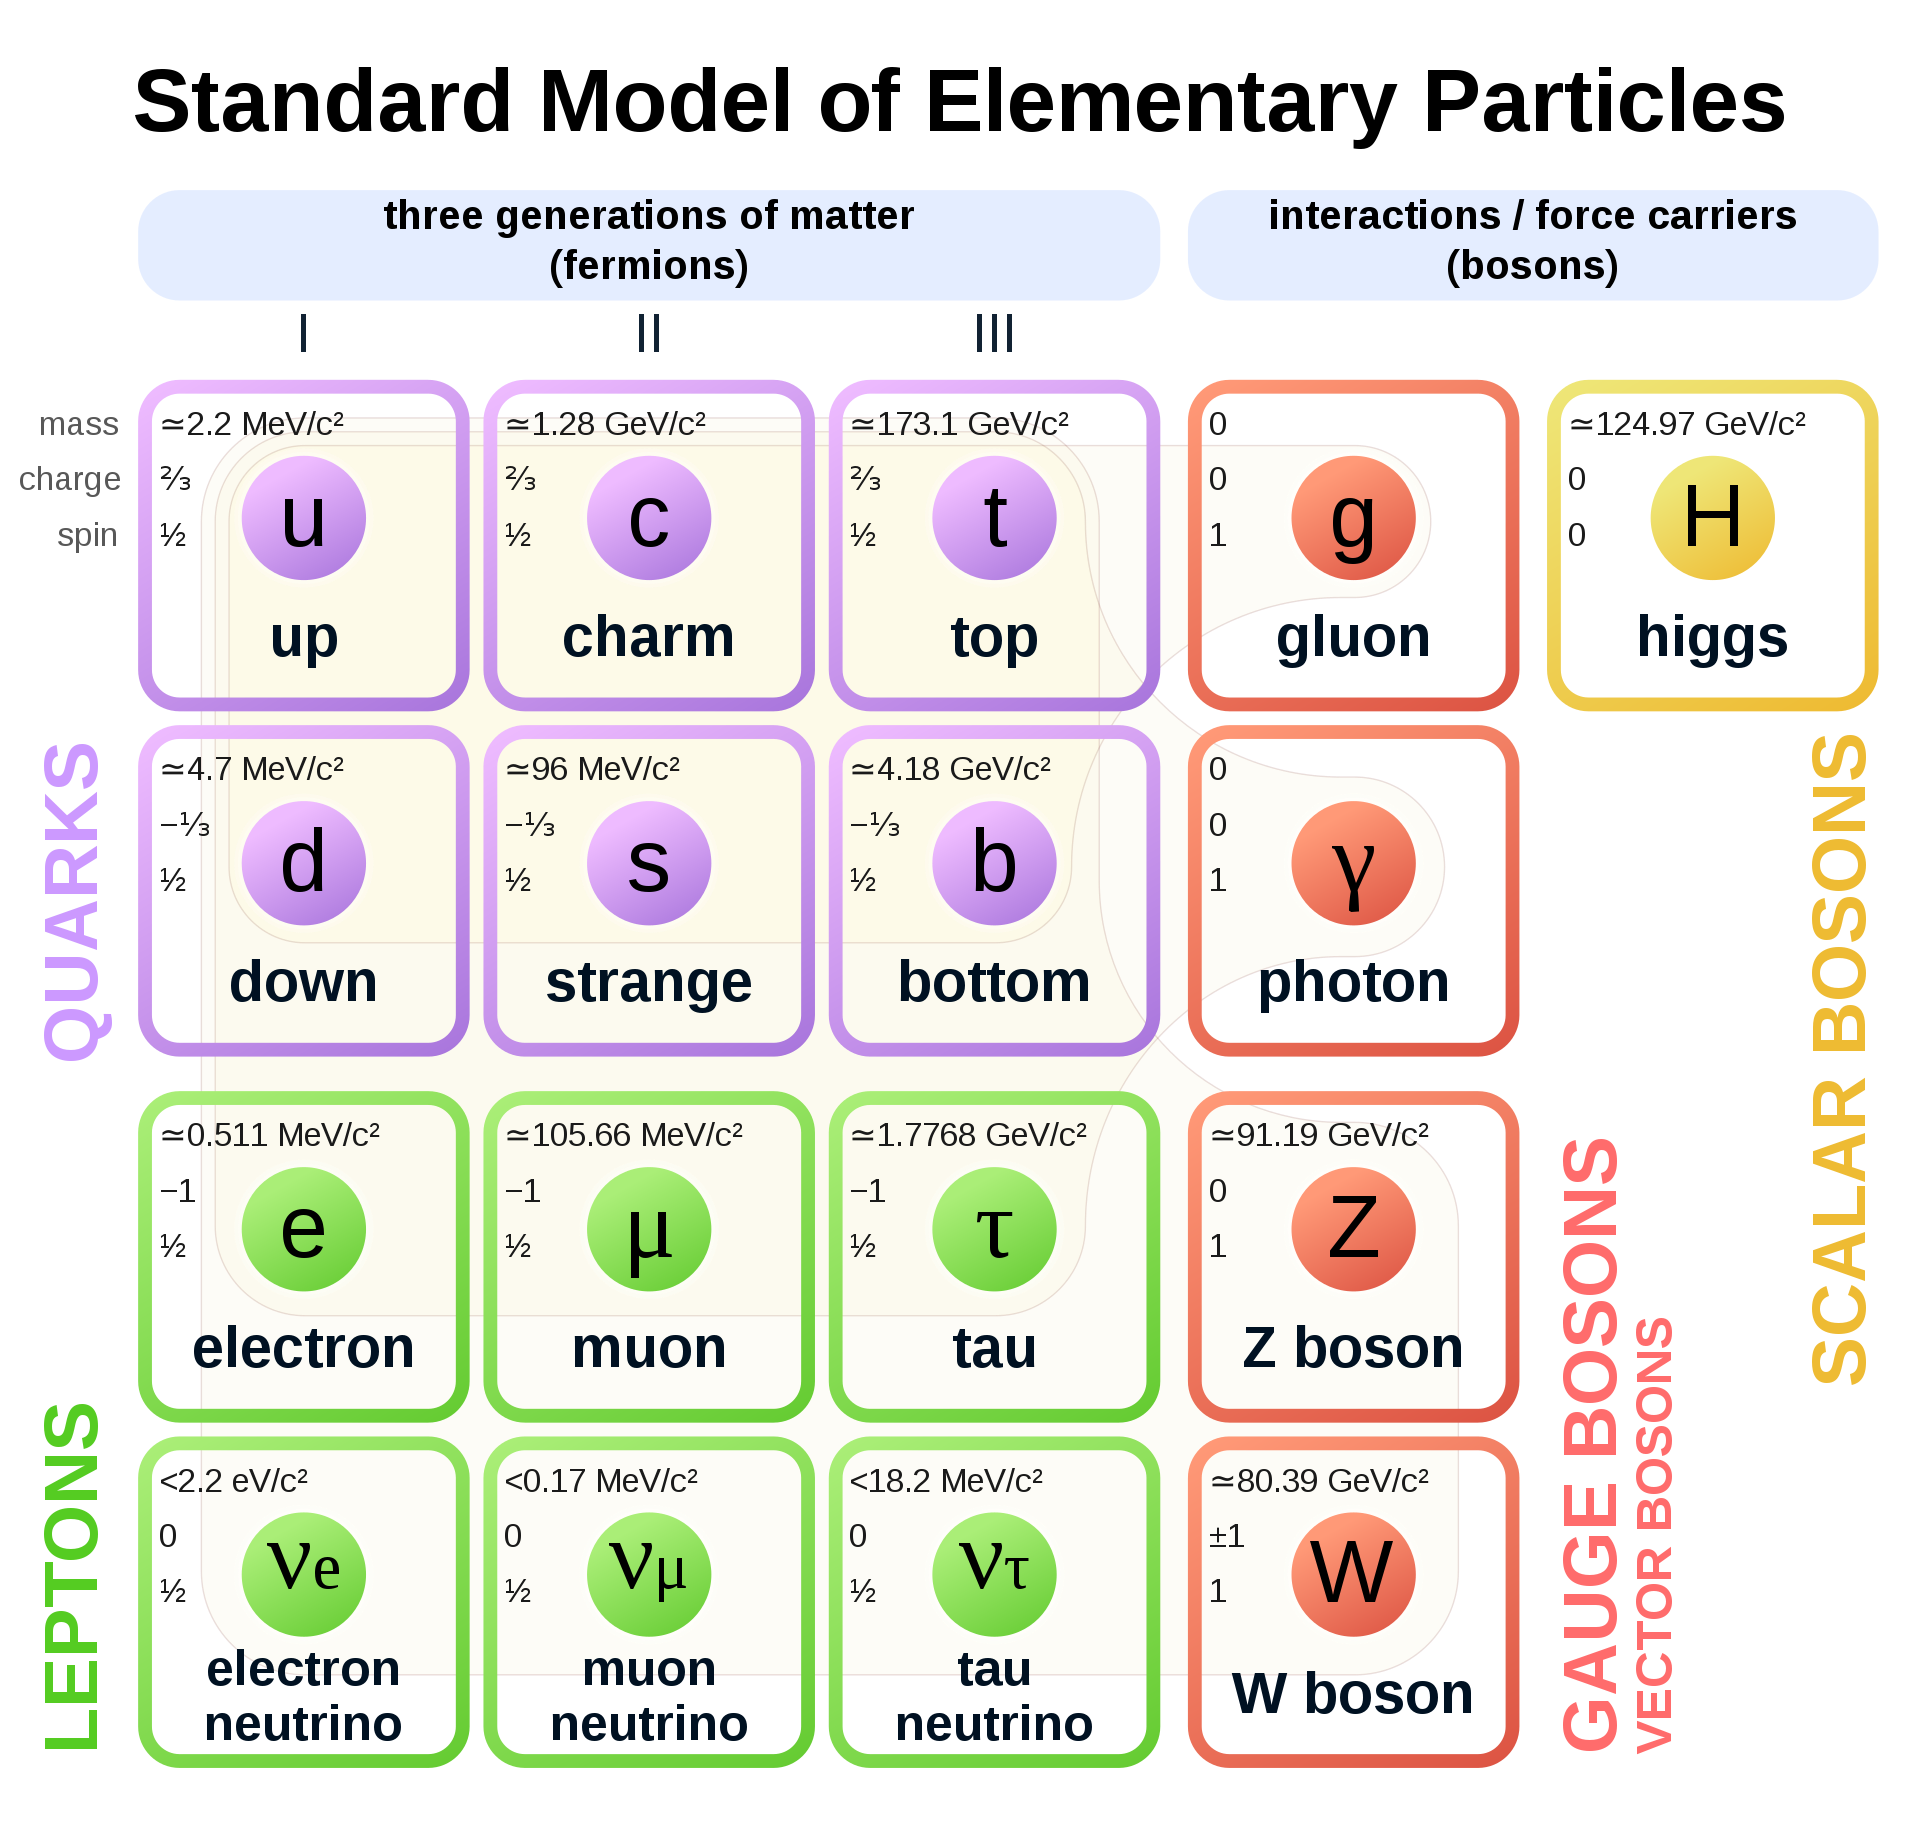
\includegraphics[width=0.8\linewidth]{fig/standard_model.png}
    \captionof{figure}{Standard Model of particle physics.}
    \end{center}

There are three different interactions which are mediated by bosons carrying spin $1$.
The exchange particles of the weak force are the massive $Z$ and $W^{\pm}$ bosons, the massless photons for the electromagnetic force and eight massless gluons are mediating the strong force. 
The main interest of this experiment lies in the $Z$ boson.
Its properties are shown in table \ref{table:zboson}:
        \begin{center}
            \begin{tabular*}{\linewidth}{c c c}
        \toprule
                Charge & Mass \si{[GeV]} & $\Gamma$\si{[GeV]}\\%Decay Width \si{[GeV]} \\ 
        \midrule
                \small{0} & \small {$91.1876 \pm 0.0021$} & \small{$2.4952 \pm 0.0023$} \\
        \bottomrule
    \end{tabular*}
            \captionof{table}{Properties of the $Z$ Boson.}
        \label{table:zboson}
        \end{center}


\subsection{Drell-Yan Process}
A $Z$ Boson can be created during the so called ``Drell-Yan'' process (fig. \ref{fig:drell_yan}). 

    \begin{center}
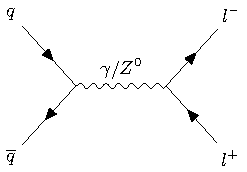
\includegraphics[width=0.55\linewidth]{fig/feynman_0.pdf}
        \captionof{figure}{Drell-Yan process.}
\label{fig:drell_yan}
\end{center}

This process happens in proton-proton collisions.
When a quark and an anti-quark collide either a virtual photon $\gamma^\ast$ or a $Z$ Boson can be produced. 
The $\gamma^\ast$ or the $Z$ can then split into a lepton and its anti-particle partner, like electron-positron or muon and anti-muon.
The sum of the lepton and anti-particle partner momenta will then add up to the former boson momentum. 
A peak around $90$ \si{GeV} will be observed corresponding to the $Z$ boson. 

\subsection{ATLAS Detector}
\subsubsection{Components}
The detector consists of three main components: inner detector, calorimeters and the muon spectrometer.
They are onion-like constructed. 
The inner detector, the innermost layer, is mainly used to reconstruct the trajectories of electrically charged particles and to determine their momenta. 
With three also onion-like ordered tracking detectors, the pixel detector, the semi-conductor tracker and the transition radiation tracker, the inner detector can measure charged particles in a range of $\abs{\eta} < 2.5$ and a $p_{T} > 400$ \si{MeV}.\\

The electromagnetic and the hadronic calorimeter allow to reconstruct the shapes of the showers from electromagnetically and strongly interacting particles. 
They are designed to contain the whole shower and cover a range of up to $\abs{\eta} < 4.9$. 
A precise energy measurement is possible.\\
The outermost layer is the muon spectrometer used for tracking Muons.

\subsubsection{Geometry of the Detector}
In figure \ref{fig:cross_section_detector} one can see a image of the cross section of the ATLAS detector, which has a rotational symmetry around the $z$-axis.
\begin{center}
	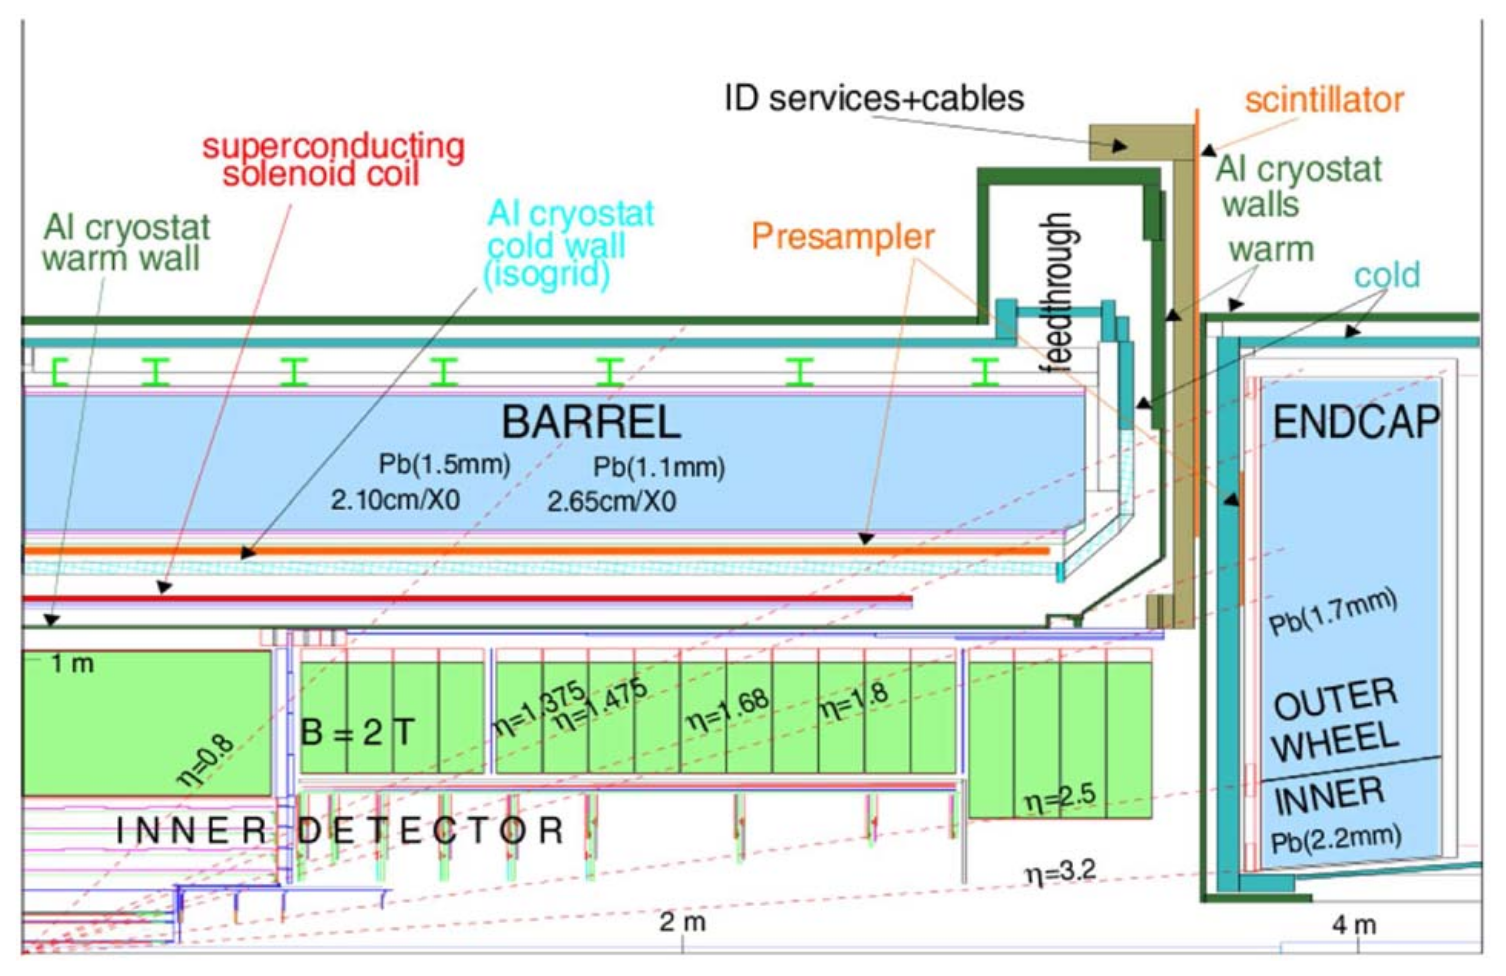
\includegraphics[width=0.8\linewidth]{fig/detector_geometry.png}
	\captionof{figure}{Cross section of the ATLAS detector.}
	\label{fig:cross_section_detector}
\end{center}
A good understanding of the detector geometry is necessary to compute the $Z$ bosons mass later on. 
One introduces the so called pseudo-rapidity $\eta$
\begin{align}
    \eta = - \log \tan \left( \frac{\theta}{2} \right).
\end{align}
The components of the momentum of a given particle are
\begin{align}
    p_x = p_T \cos \phi , \\
    p_y = p_T \sin \phi ,
\end{align}
where $p_T$ is the transversal momentum.
By using the $\eta$ definition one can derive $p_z$ in the following way
\begin{align}
    & p_z = p_t \cot \theta , \\
    & \text{use: } \cot (2\arctan \e^{-x}) = \sinh x , \\
    \Rightarrow \ & p_z = p_T \sinh \eta .
\end{align}
%\begin{center}
%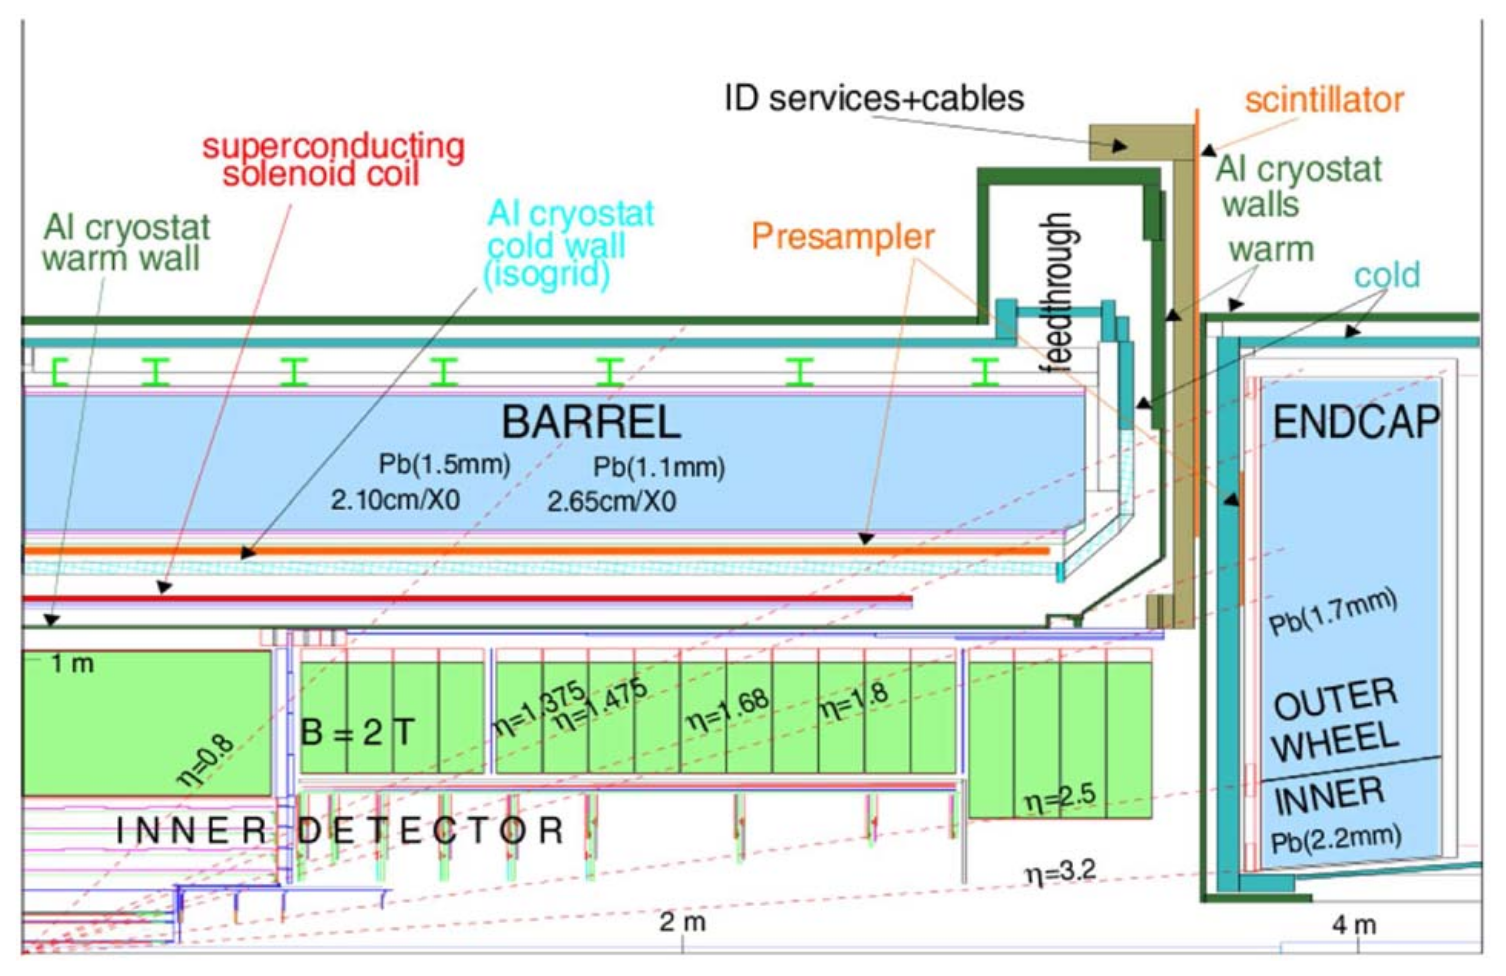
\includegraphics[width=0.8\linewidth]{fig/detector_geometry.png}
%        \captionof{figure}{Cross section of the ATLAS detector.}
%\label{fig:cross_section_detector}
%\end{center}

\subsection{Distributions}
For the experiment the following distributions are important.\\
\textbf{Gaussian distribution}
\begin{align}
    f_{\text{G}} (E) = \frac{\mathcal{N}}{\sqrt{2 \pi \sigma^2}} \exp \left( - \frac{(E - \mu )^2}{2 \sigma^2} \right)
\end{align}
\textbf{Breit-Wigner Distribution}
\begin{align}
    f_{\text{BW}} = \frac{\mathcal{N} k}{(E^2 - M^2)^2 + M^2 \Gamma^2} ,
\end{align}
where $k = \frac{M\Gamma \gamma \sqrt{8}}{\pi \sqrt{M^2 + \gamma}}$ and $\gamma = M \sqrt{M^2 + \Gamma^2}$. $\Gamma$ is the decay width.\\
One also needs a third distributions which is the \textit{convolution} of the Gauss and the Breit-Wigner Distribution in order to account for the finite energy resolution of the detector. 
The Breit-Wigner describes the physical decay process. 
However, it does not consider the energy uncertainties which can be accounted for by the Gaussian distribution.
A convolution of two functions $(f \ast g)$ is defined as:
\begin{align}
    (f \ast g) (x) = \int f(y)g(x-y)\dd y
\end{align}

\subsection{Efficiency}
Another important part of evaluating the data is to estimate the efficiencies of the different triggers.
At the ATLAS detector it consists of four components:
\begin{align}
     \epsilon_{\text{tot}} =  \epsilon_{\text{recon}} \times \epsilon_{\text{id}} \times \epsilon_{\text{trig}} \times \epsilon_{\text{add}}  .
\end{align}
The focus of this experiment lies on the identification efficiency.
One can get an estimate for $\epsilon_{\text{id}}$ by using the so called tag and probe method.
One searches for one event where two electrons are involved. 
Now strict conditions are applied on one of the electrons, the \textit{tag} electron, 
and on the other one, the \textit{probe} electron, weaker conditions are applied.
Let $N_{tp}$ be the number of events where both tag and probe fulfill their conditions and $N_t$ be the number of events where the tag electron passes the requirements and where tag and probe electron pass the requirements, then the efficiency is given by:
\begin{align}
    \epsilon_{\text{id}} = \frac{N_{tp} (p_T)}{N_t(p_T)}.
\end{align}


\section{Experimental Procedure}

\subsection{Getting Familiar with the Data}
Before starting with the analysis one has to make oneself familiar with the provided data and \verb*+ROOT+.
One only has data from events where a primary vertex was found and at least one lepton has a minimal transverse momentum of $p_{T} = 25$ \si{GeV}.

\subsubsection{Position of Particle Collisions}
\begin{center}
	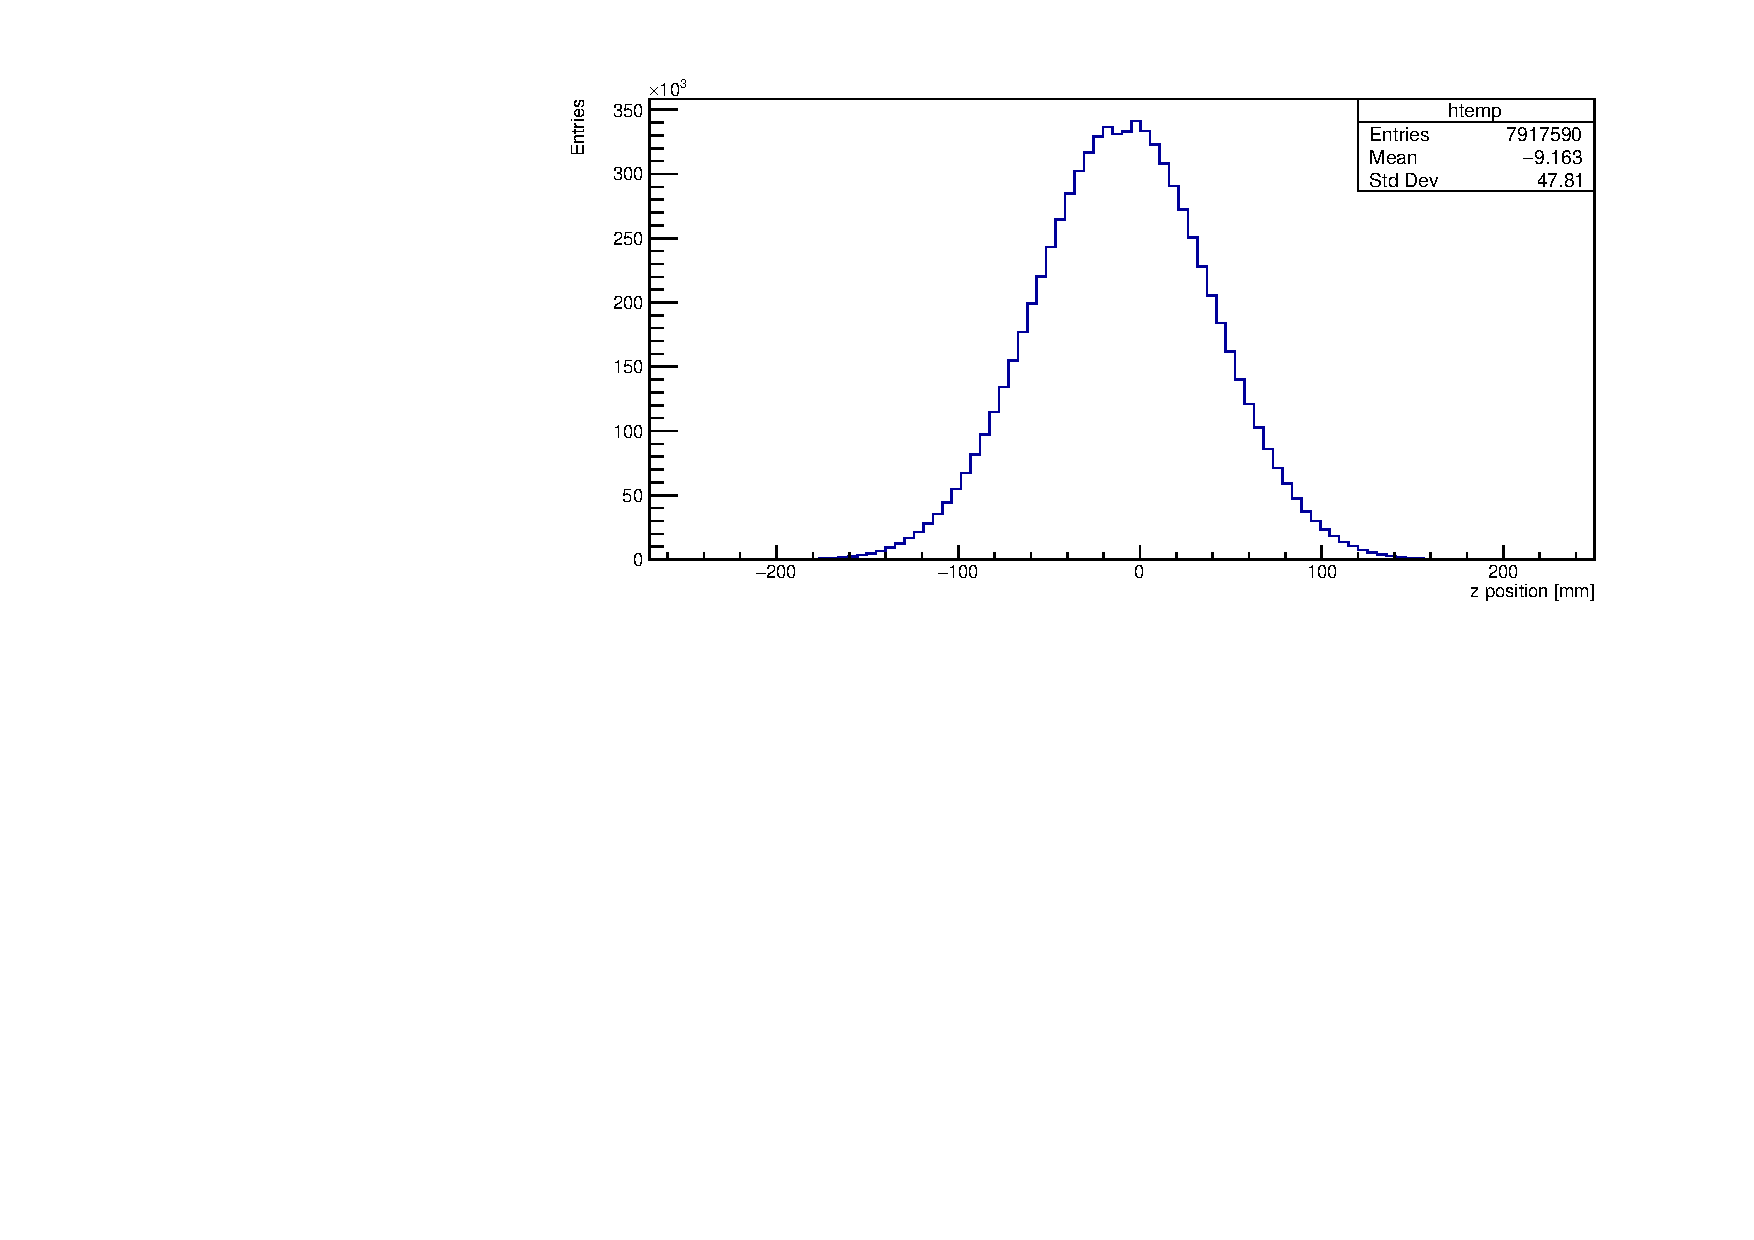
\includegraphics[width=\linewidth]{fig/vxp_z_final.pdf}
    \captionof{figure}{Distribution of collisions along the $z$ axis.}
	\label{vxp_z}
\end{center}
To check where the particle collisions occur, one can evaluate the given data for the $vxp_z$ variable. 
The results are shown in figure \ref{vxp_z}.
The mean is shifted by $-9$ \si{mm}. 
This confirms, that the given data is from 2012, because collisions of bunches were not calibrated to the $0.0$ position back then \cite{atlasbeamspot}.
There are two maxima which can also be explained with the assumption above. 

\subsubsection{leptons per event}

\begin{center}
	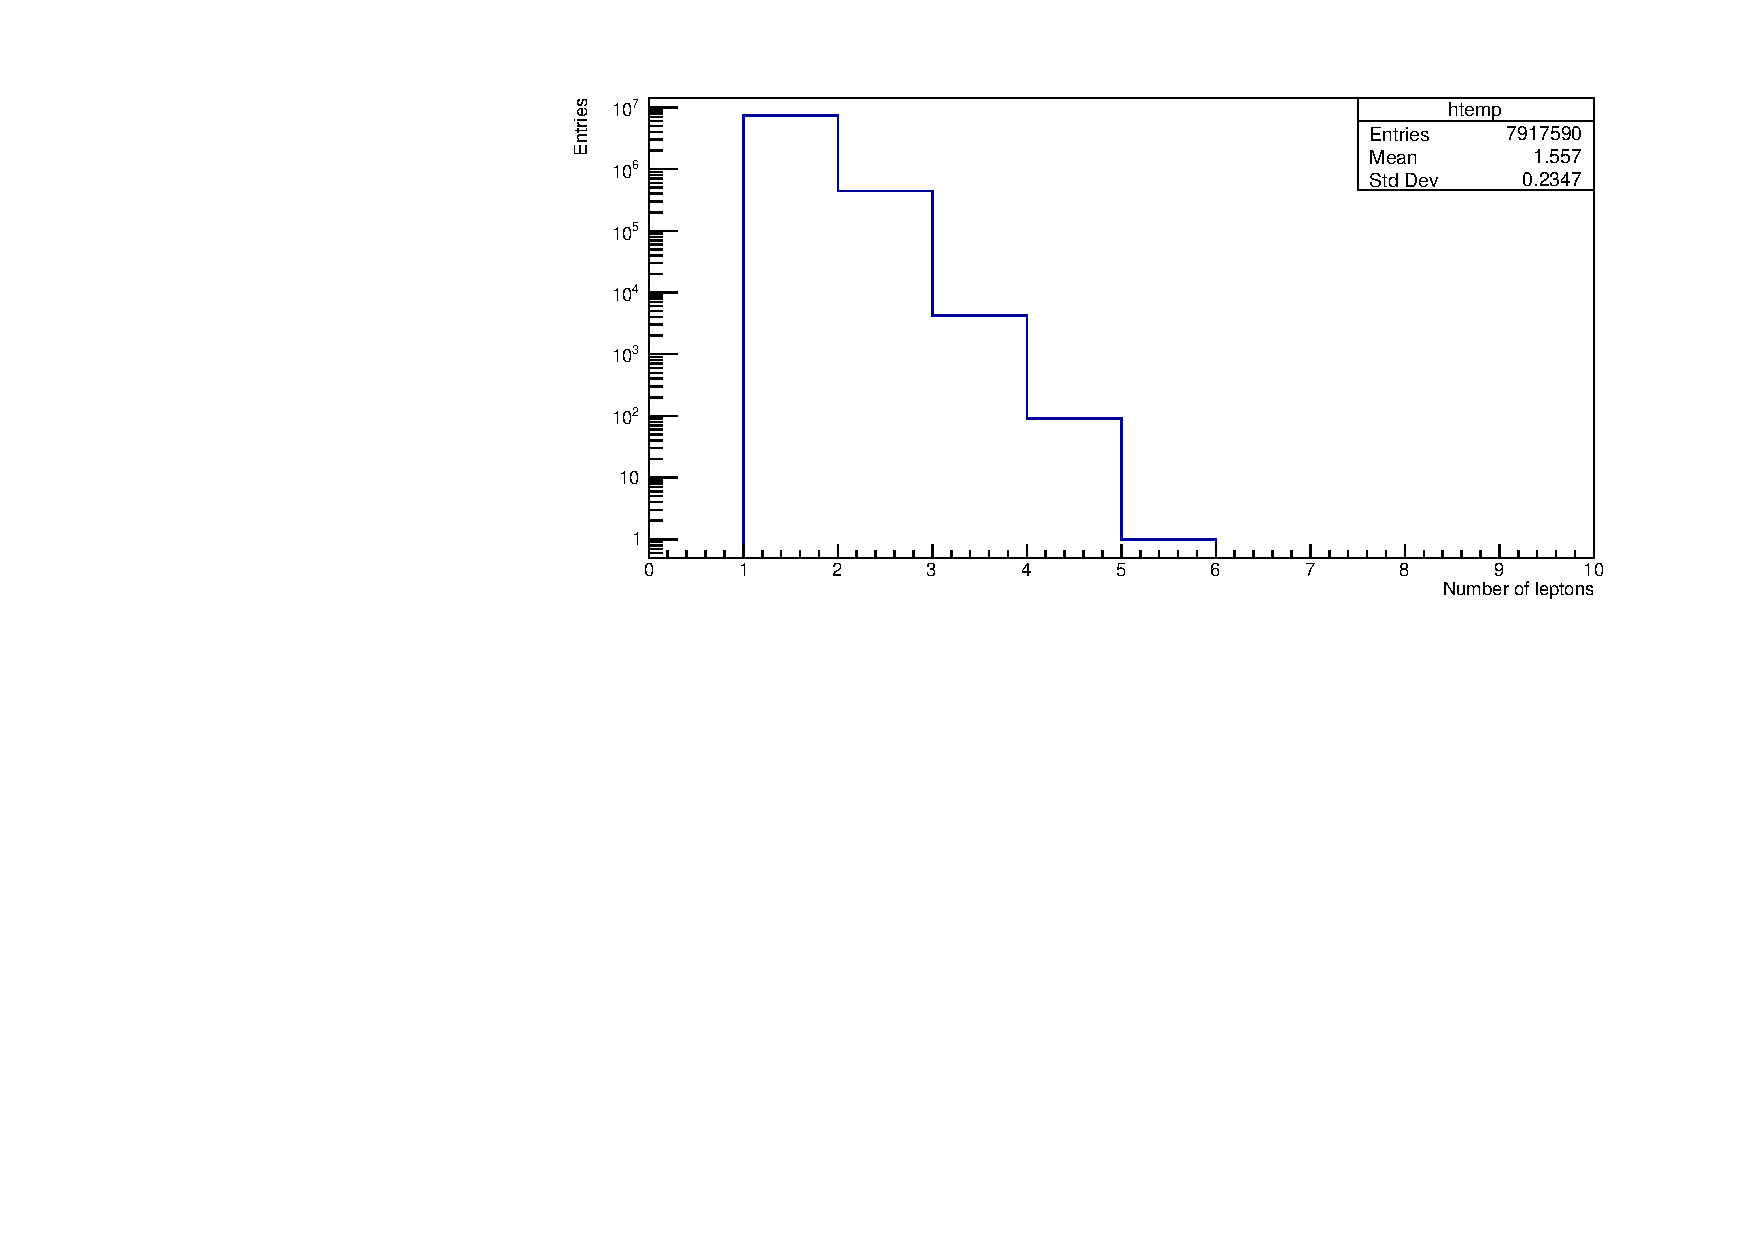
\includegraphics[width=\linewidth]{fig/lep_n_final.pdf}
    \captionof{figure}{Leptons recorded per event.}
	\label{lep_n}
\end{center}

To figure out, if one found a $Z$ decay, one analyzes the \textit{leptons per event} value of the data (fig. \ref{lep_n}).
Around the wanted two leptons, one gets many events with one and three leptons. 
For these events to happen, one needs a $W^{\pm}$ decay.
Possible decays are shown in figure \ref{fig:three_lepton}.
    \begin{center}
        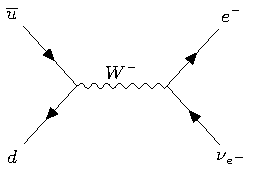
\includegraphics[width=0.45\linewidth]{fig/feynman_1.pdf} \hfill
        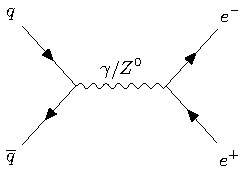
\includegraphics[width=0.45\linewidth]{fig/feynman_2.pdf} \\
        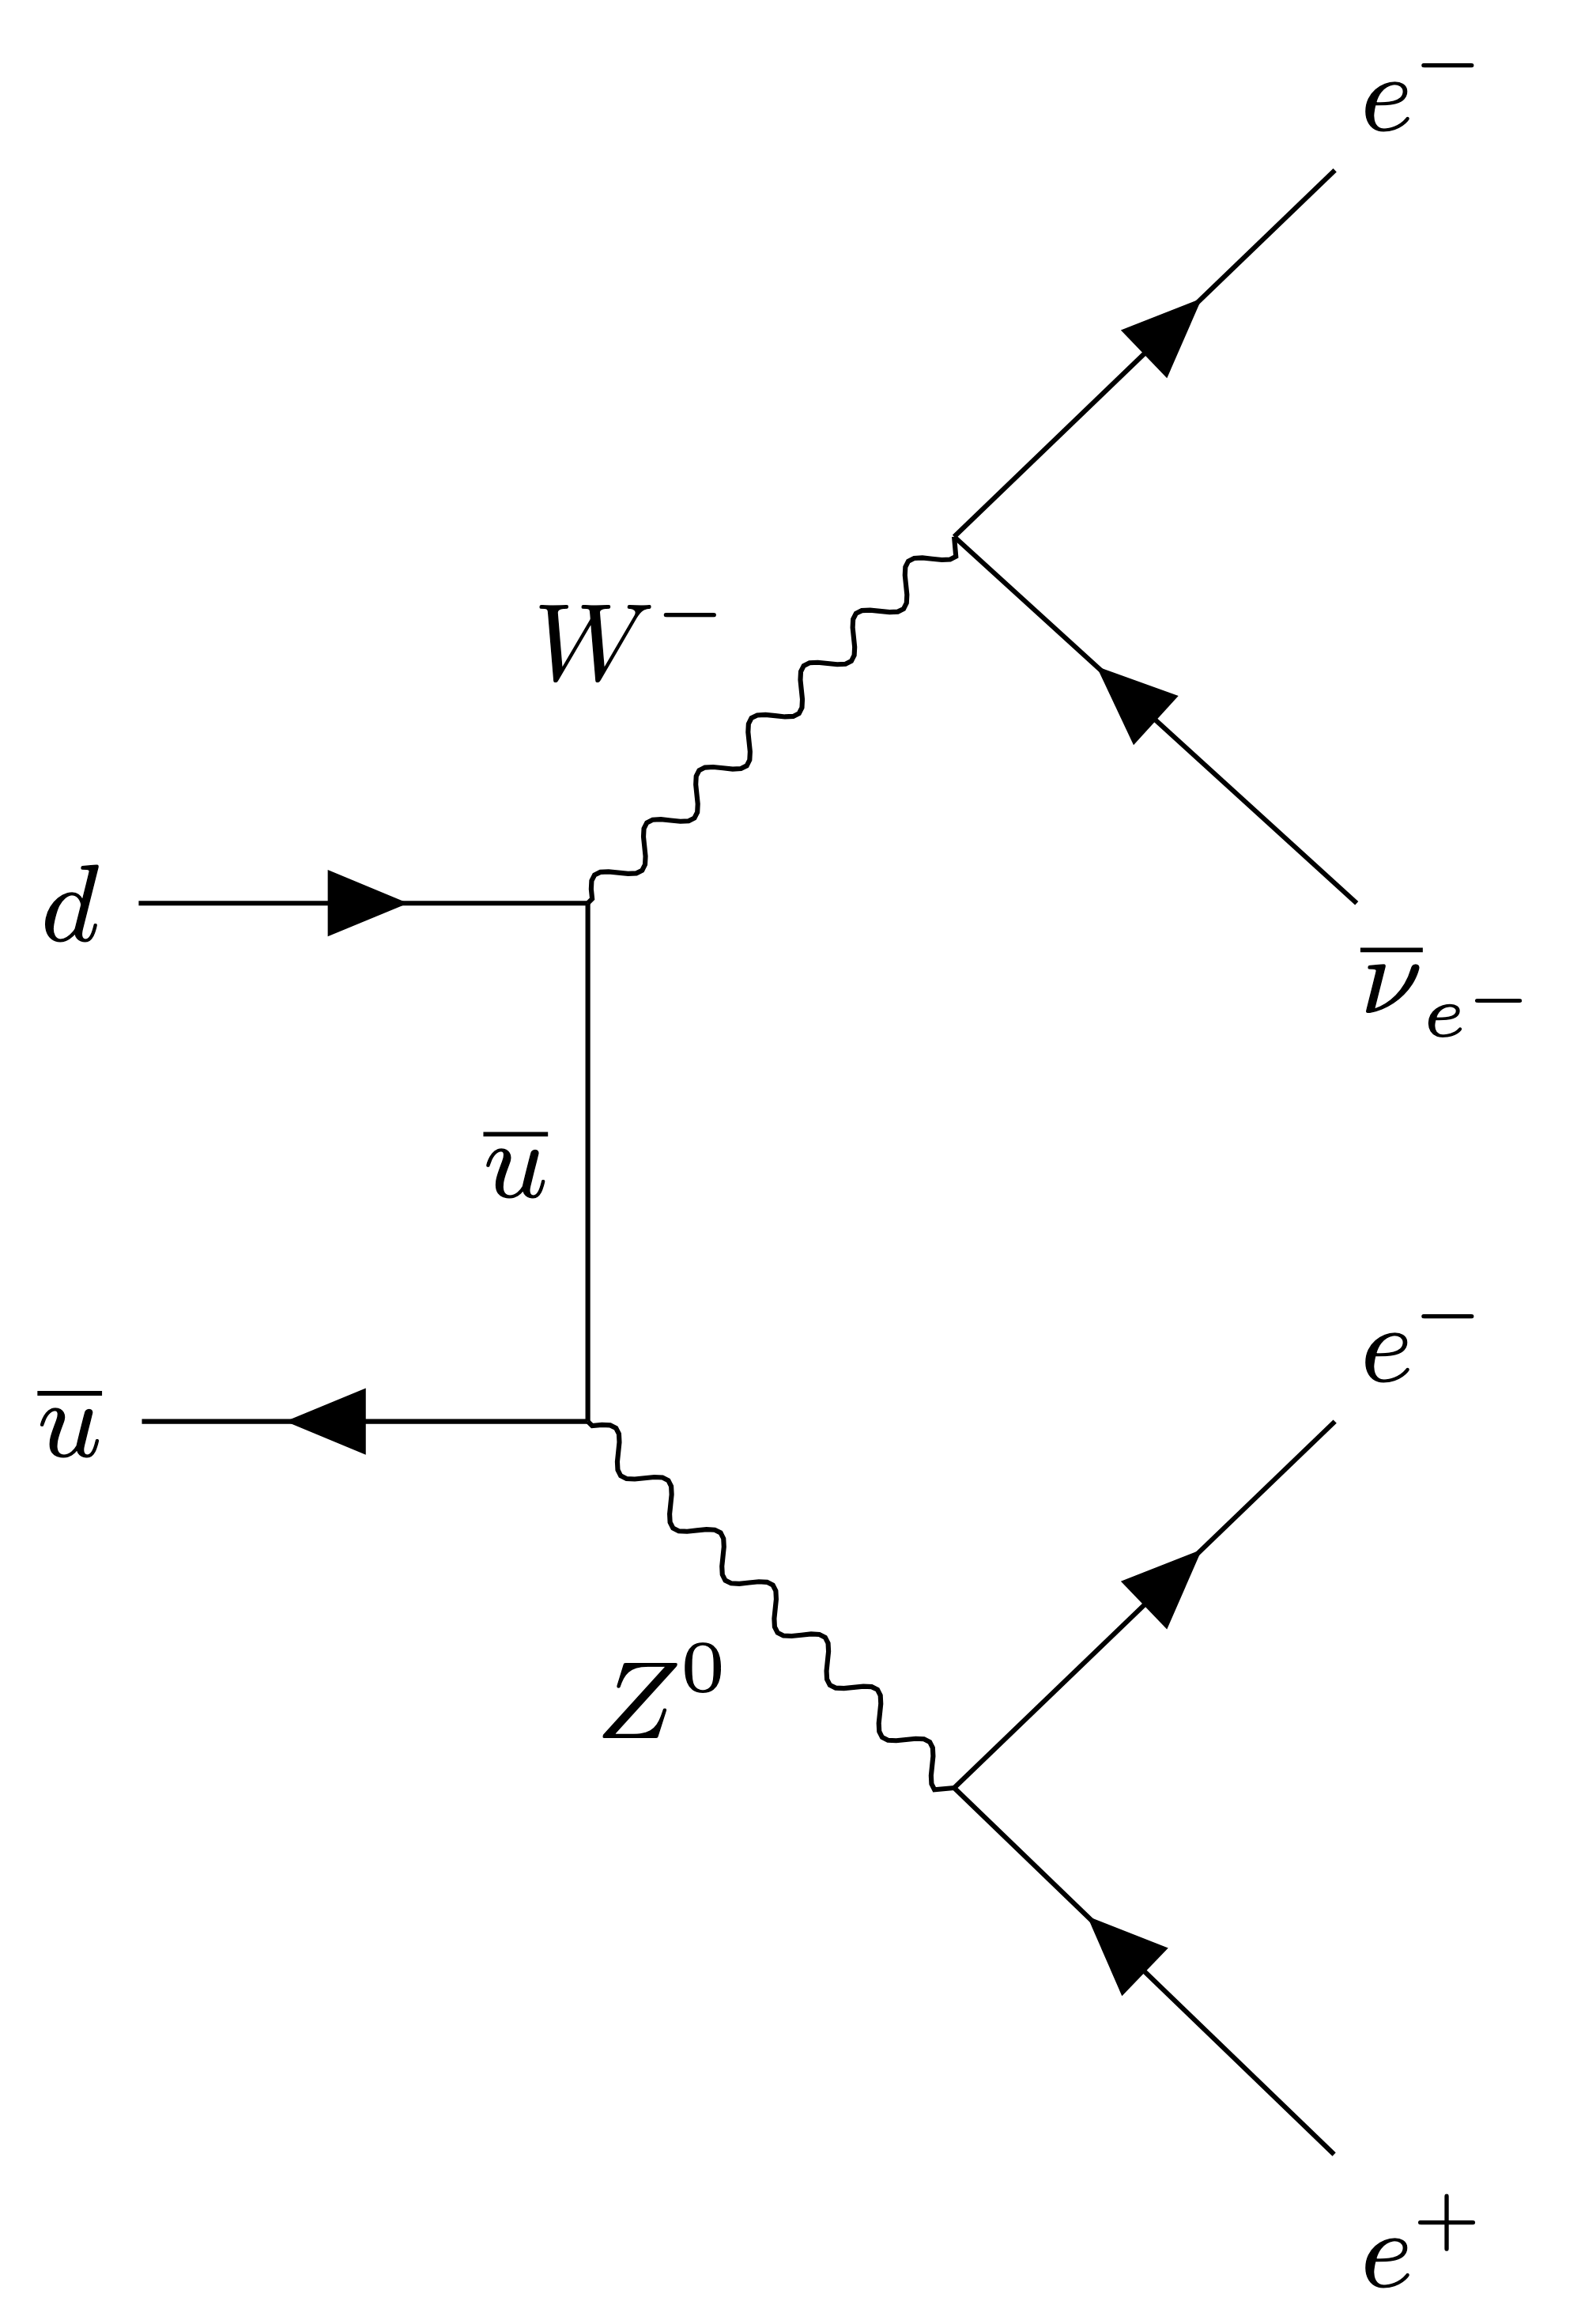
\includegraphics[width=0.45\linewidth]{fig/feynman_3.png}
\captionof{figure}{Feynman graphs for final states with one to three leptons.}
\label{fig:three_lepton}
\end{center}

\subsubsection{Lepton Kinematics}
One can identify a sharp rise at $25$ \si{GeV} for the transverse momentum. 
At ATLAS only events with at least one lepton above this threshold will be stored.
\begin{center}
    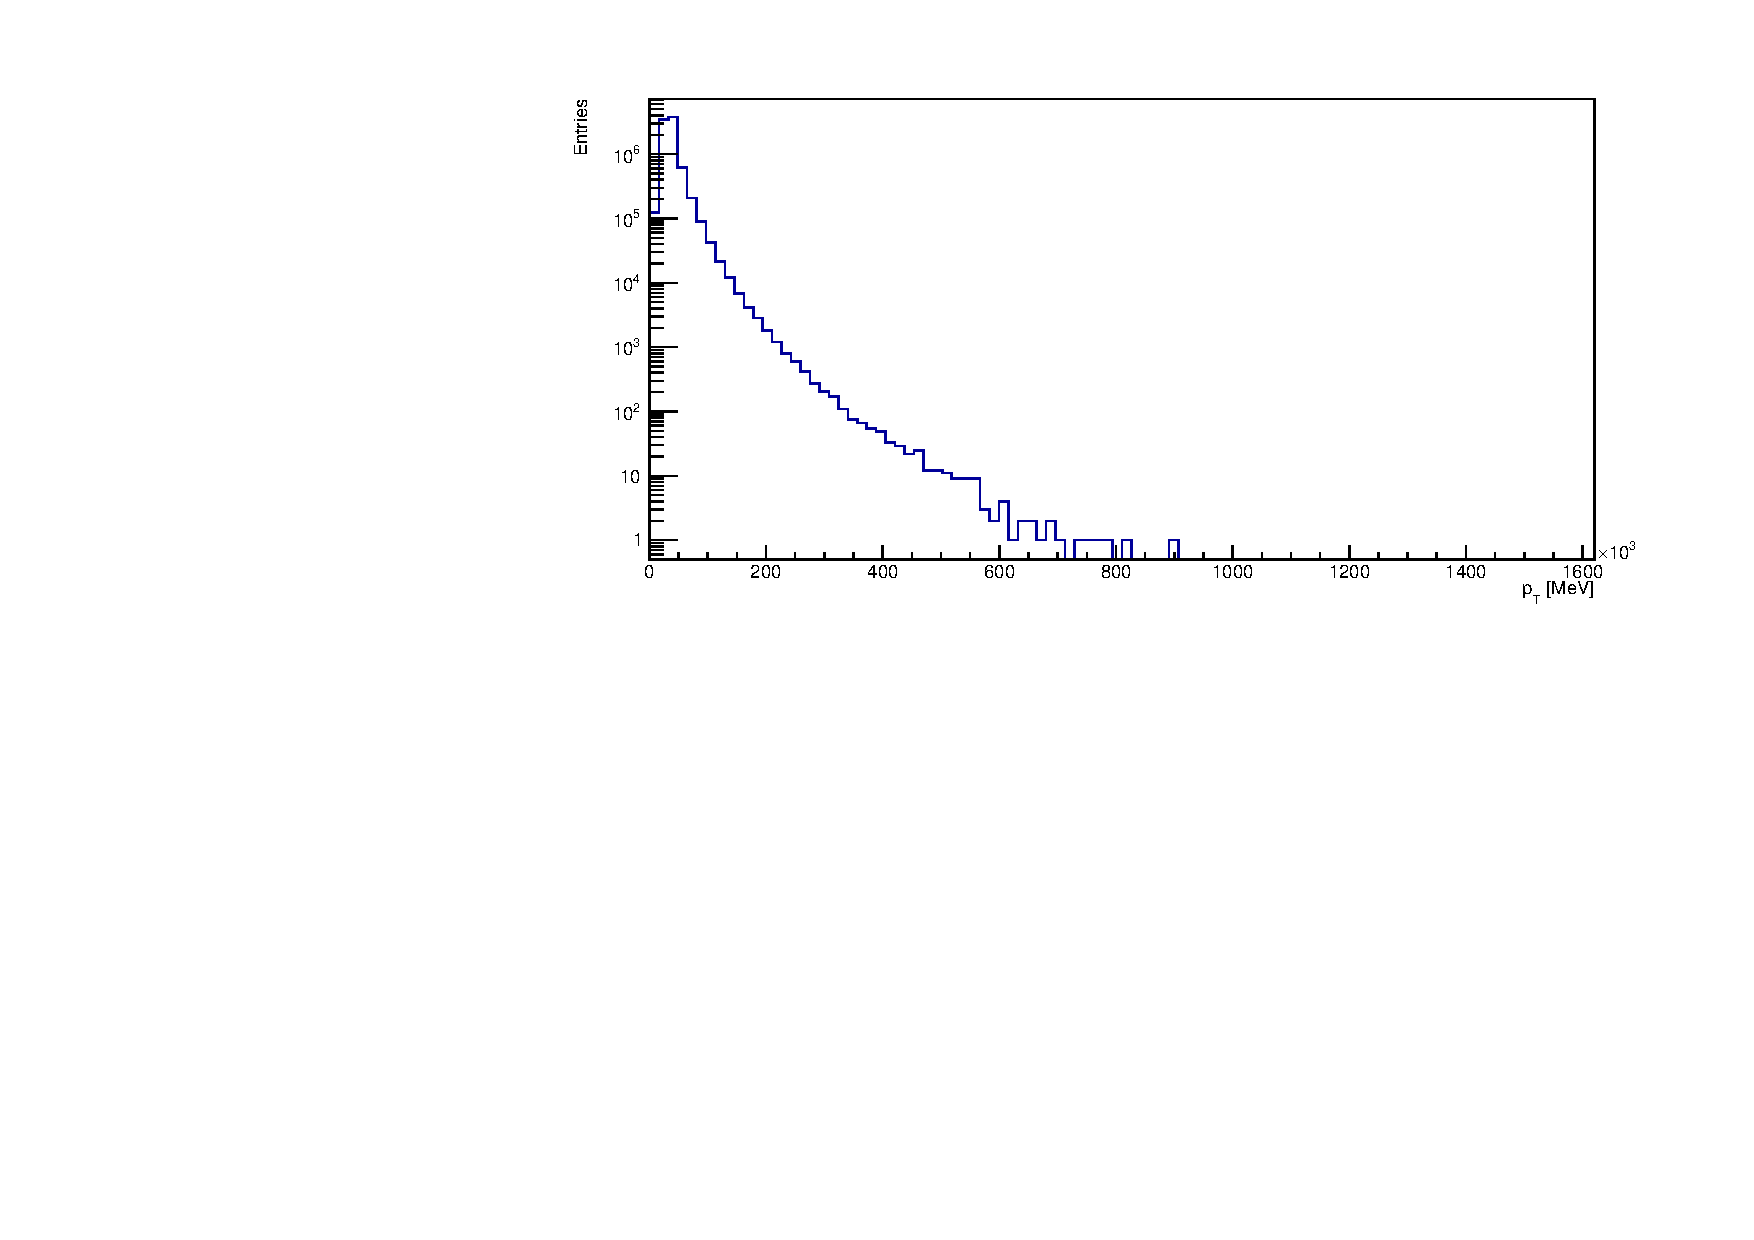
\includegraphics[width=0.8\linewidth]{fig/p_T_final.pdf}
    \captionof{figure}{Distributions of $p_T$.}
\end{center}    
The stored data (the $\phi$ angle and the $\eta$ variable) gives insight about the geometry.
\begin{center}
    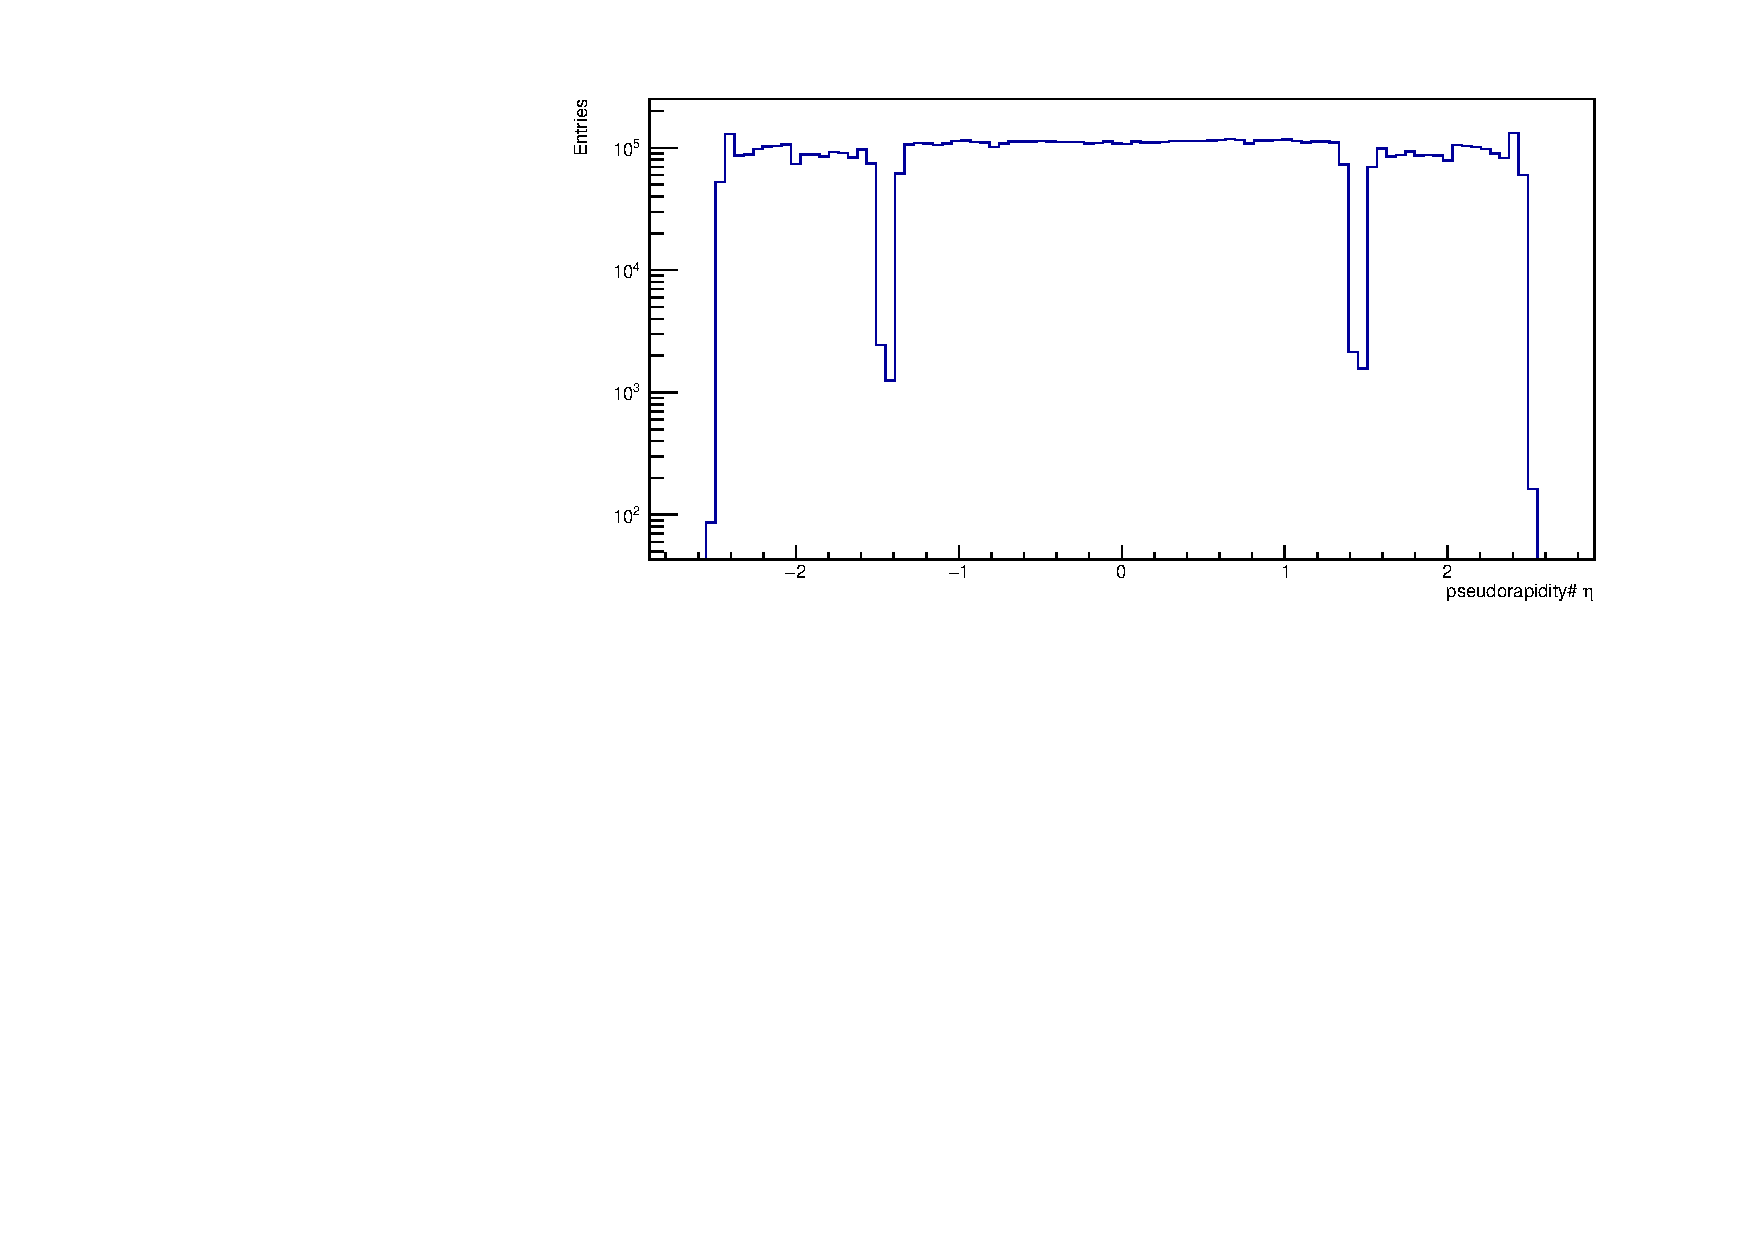
\includegraphics[width=0.8\linewidth]{fig/eta_final.pdf}
    \captionof{figure}{Distribution of $\eta$.} 
\end{center}
From the geometry one assumes an even distribution for the $\phi$ and $\eta$ values.
It only applies for the first. 
The $\eta$ value has areas with a lack of data entries. 
This is a setback of the ATLAS geometry seen in figure \ref{fig:cross_section_detector}. 
Around $\eta = 1.5$, one misses the \textit{Barrel} or the \textit{Endcap} which are necessary for the event recognition. 

\subsection{Calculation of the invariant mass of the $Z$ boson}
According to the structure of the ATLAS detector, one can calculate the invariant mass in the following way

\begin{align}
	M_{\mu} &= \sqrt{p_{\mu}p^{\mu}}. 
			%&= \sqrt{E_{1}E_{2}-p_{T_{1}}p_{T_{2}} (\cos(\varphi_{1})\cos(\varphi_{2})+\sin(\varphi_{1})\sin(\varphi_{2})+\sinh(\eta_{1})\sinh(\eta_{2}))} .
\end{align}
An attempt to calculate it with the above given formula and the build-in function \verb*+TLorenz+ in \verb*+ROOT+ provided the exact same result. 
The calculated results will therefore be based on the \verb*+ROOT+ method.

The first attempt to measure the mass was done by limiting the data to $2$-lepton events. 
Furthermore, one ignored the events where $M_{\mu}^{2} < 0$. 
\begin{center}
	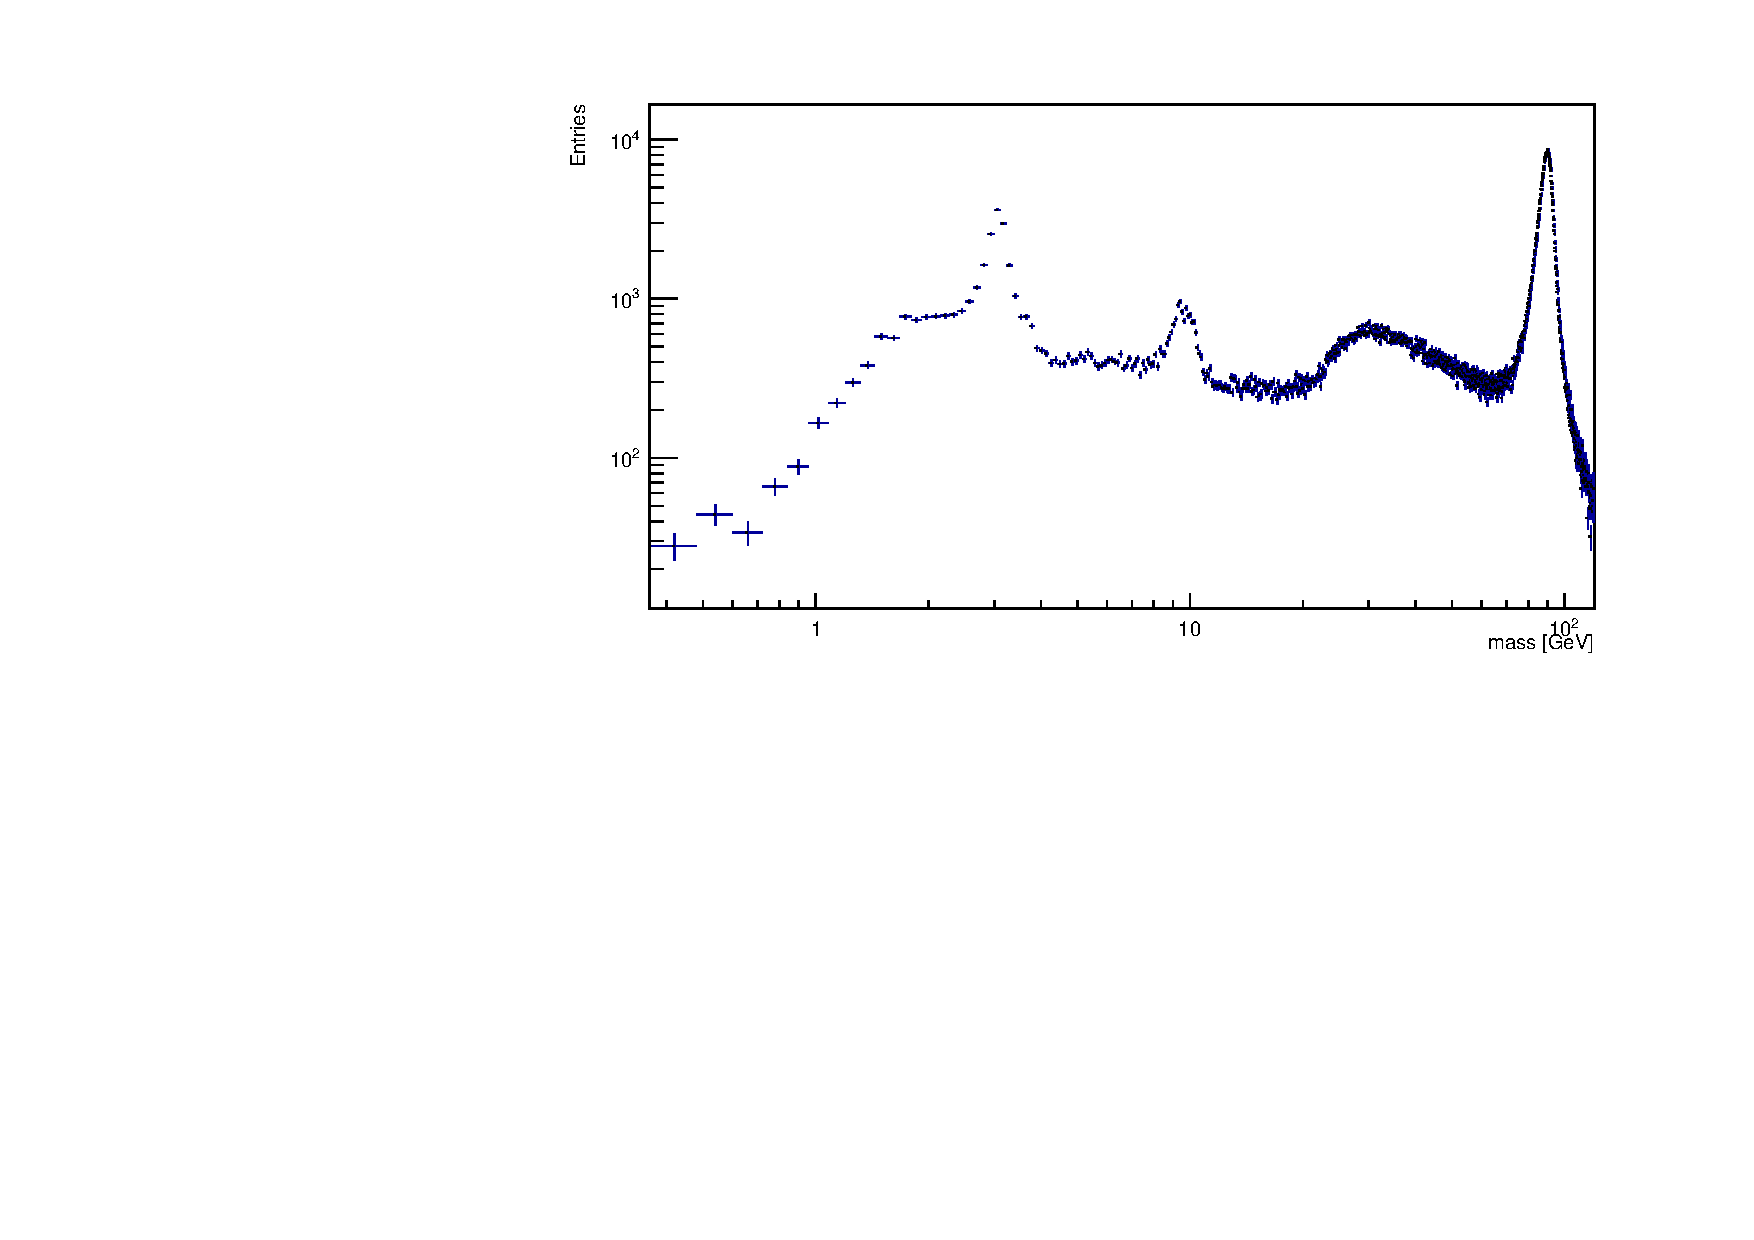
\includegraphics[width=\linewidth]{fig/invar_mass_dist_corrected_axis_title.pdf}
    \captionof{figure}{Invariant Mass distribution of 2 lepton events.}
	\label{mass_lz_log}
\end{center}

In figure \ref{mass_lz_log}, one can identify three peaks due to decay processes. 
The one on the right, at approximately $91$ \si{GeV}, is the subject of this investigation and the goal is to characterize it better in the course of this paper.\\
The one on the left is caused by the $J/{\Psi}$ and the one around $10$ \si{GeV} by the $\Upsilon$ decay. 

\subsection{Event Selection} 
The next step was to assert restrictions to the dataset in order to ensure that a $Z$ decay was measured.
The restrictions that were used are:
\begin{enumerate}
    \item \textbf{Weights}: Applies a weight to the events in the MC files, in contrast each event in real data counts as one event.
    \item \textbf{Trigger}: Events pass if the applied trigger identifies a lepton with energy above 25 \si{[GeV]}.
    \item \textbf{GRL}: The Good Run List only allows events where meaningful data for physical analysis is gathered.
    \item \textbf{Vertex}: Requires at least one well measured vertex per event.
    \item \textbf{2 Leptons}: Restrict the data to 2 lepton events.
    \item \textbf{PDGID}: A number is assigned to each particle. $e$, $\mu$ and $\tau$ are respectively identified with the integers 11, 13, and 15.
    \item \textbf{Charge}: Checks if the leptons from the $Z$ decay have opposite charge.
    \item \textbf{$p_{T}$ Cut}: Set an lower limit for the lepton energy to acknowledge the high $Z$ mass ($p_{T} > 25 \si{[GeV]}$).
    \item \textbf{Isolation}: Events pass if the observed leptons are well distinguishable from the background ($< 0.1$).
    \item \textbf{Tight ID}: Lepton reconstruction algorithms allow to label leptons. Only the ones labeled with "tight" will proceed.
    \item \textbf{Z Mass}: With the known $Z$ mass, one can restrict the mass of the di-leptons to a range around it ($70 - 110 \si{[GeV]}$). 
\end{enumerate}

The impact of each of the restrictions can be seen in figure \ref{fig:cutflow}. 
\begin{center}
	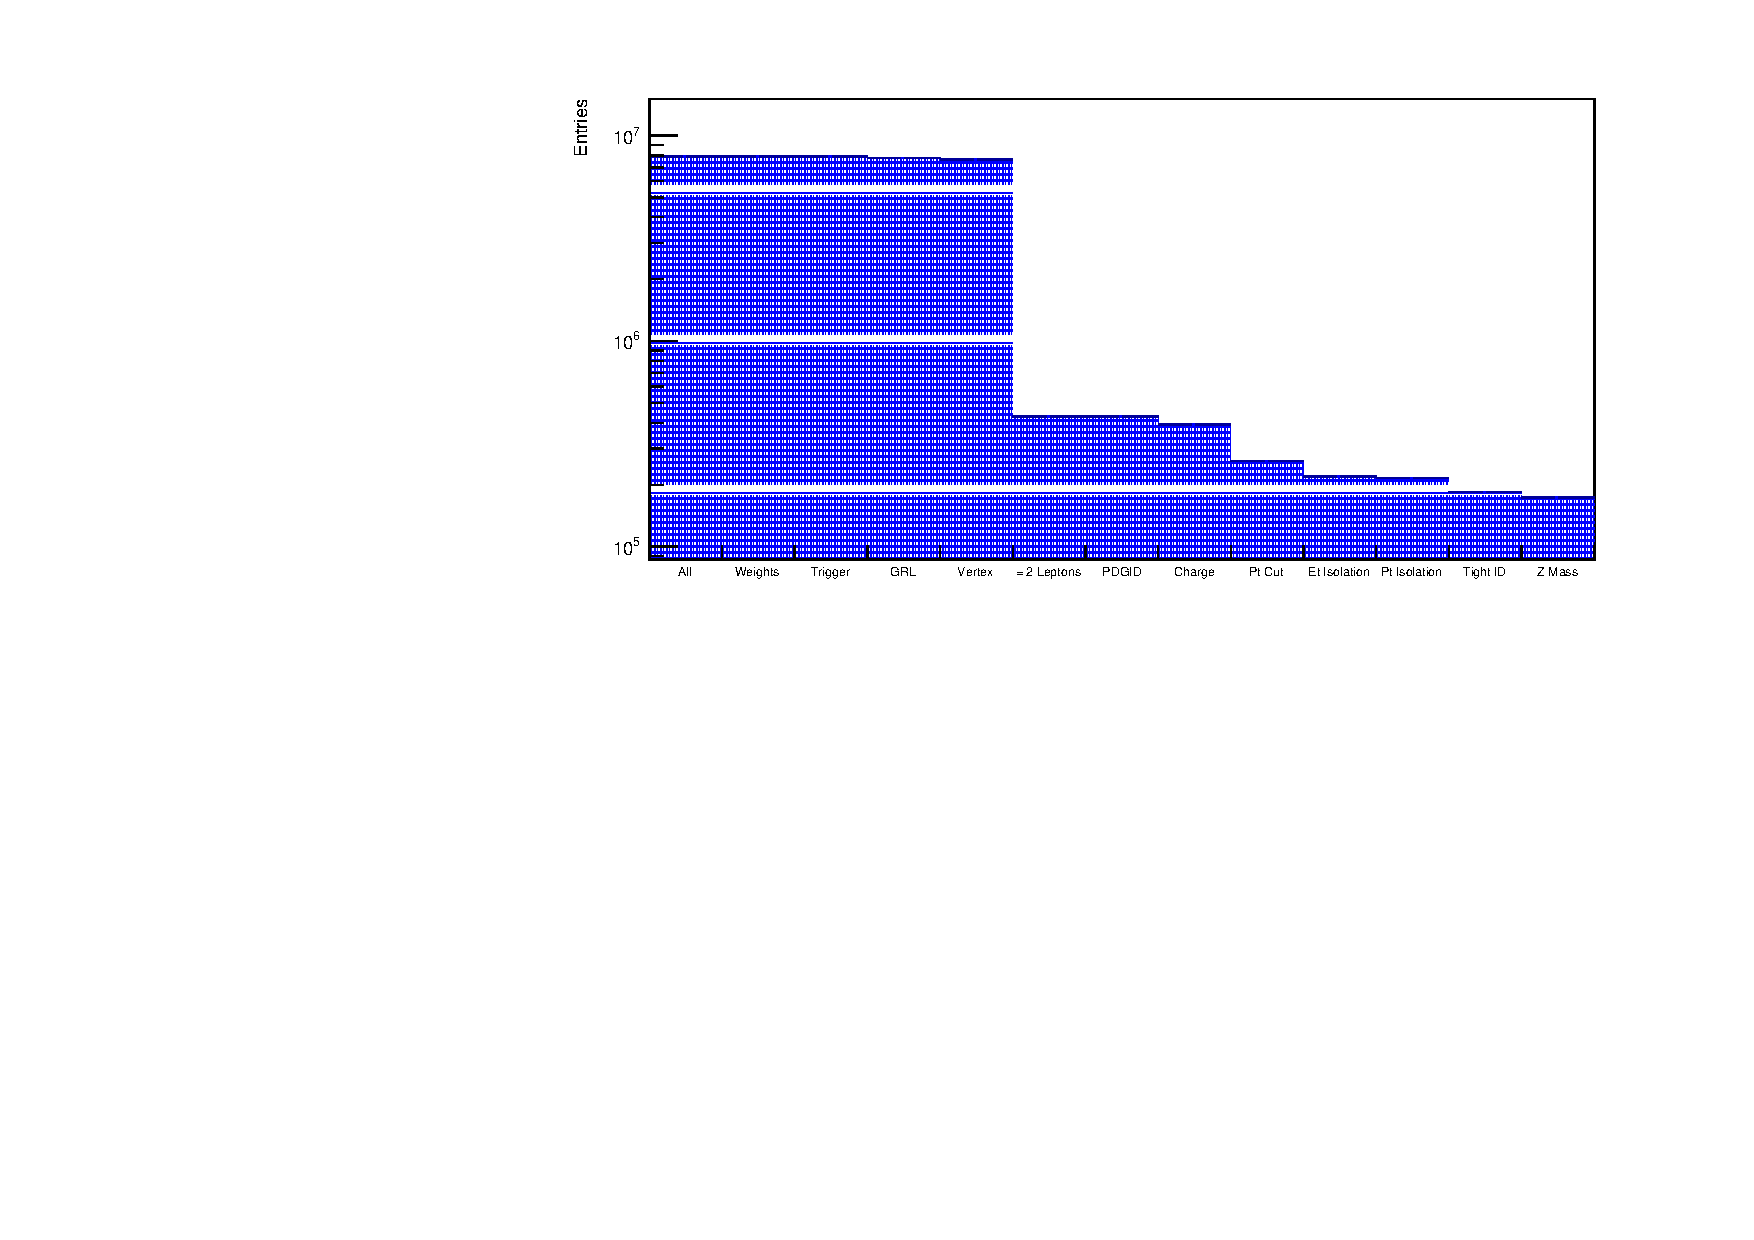
\includegraphics[width=1.1\linewidth]{fig/cutflow_hist_final.pdf}
    \captionof{figure}{cutflow histogram.}
	\label{fig:cutflow}
\end{center}
The event based cuts (in fig.\ref{fig:cutflow} the first four columns) have close to no impact on the selection because the given raw data from ATLAS is preselected on event and physics object level.
The $2$-lepton cut has the biggest impact.
As seen in figure \ref{lep_n}, most of the events do not fulfill this criteria.
%As seen, the highest cut impact provides the 2 lepton cut, which  is necessary for a $Z$ %decay. ATLAS only required one well measured primary vertex to save it as an event.
%The cut with the second highest impact is the $p_{T}$ Cut. Due to the high mass of the $Z$ %Boson, one can restrict oneself to leptons with at least $25$ GeV. The distribution of the %transvers momenta from the two decay leptons peaks around half the $Z$ mass. 


\subsection{Comparing Data and Monte Carlo Simulation}
One can now ask how well the measured data matches with the theory. 
Hence, one can perform Monte Carlo (MC) simulations and then compare with the real data (fig. \ref{fig:data_mc}). 
Three MC simulations for the possible lepton flavour after the $Z$ decay are analyzed in the same way as explained in section 2.3. 
One has to scale the results according to the luminosity of the open dataset ($1 fb^{-1}$).
The comparison yields matching results.
\begin{center}
	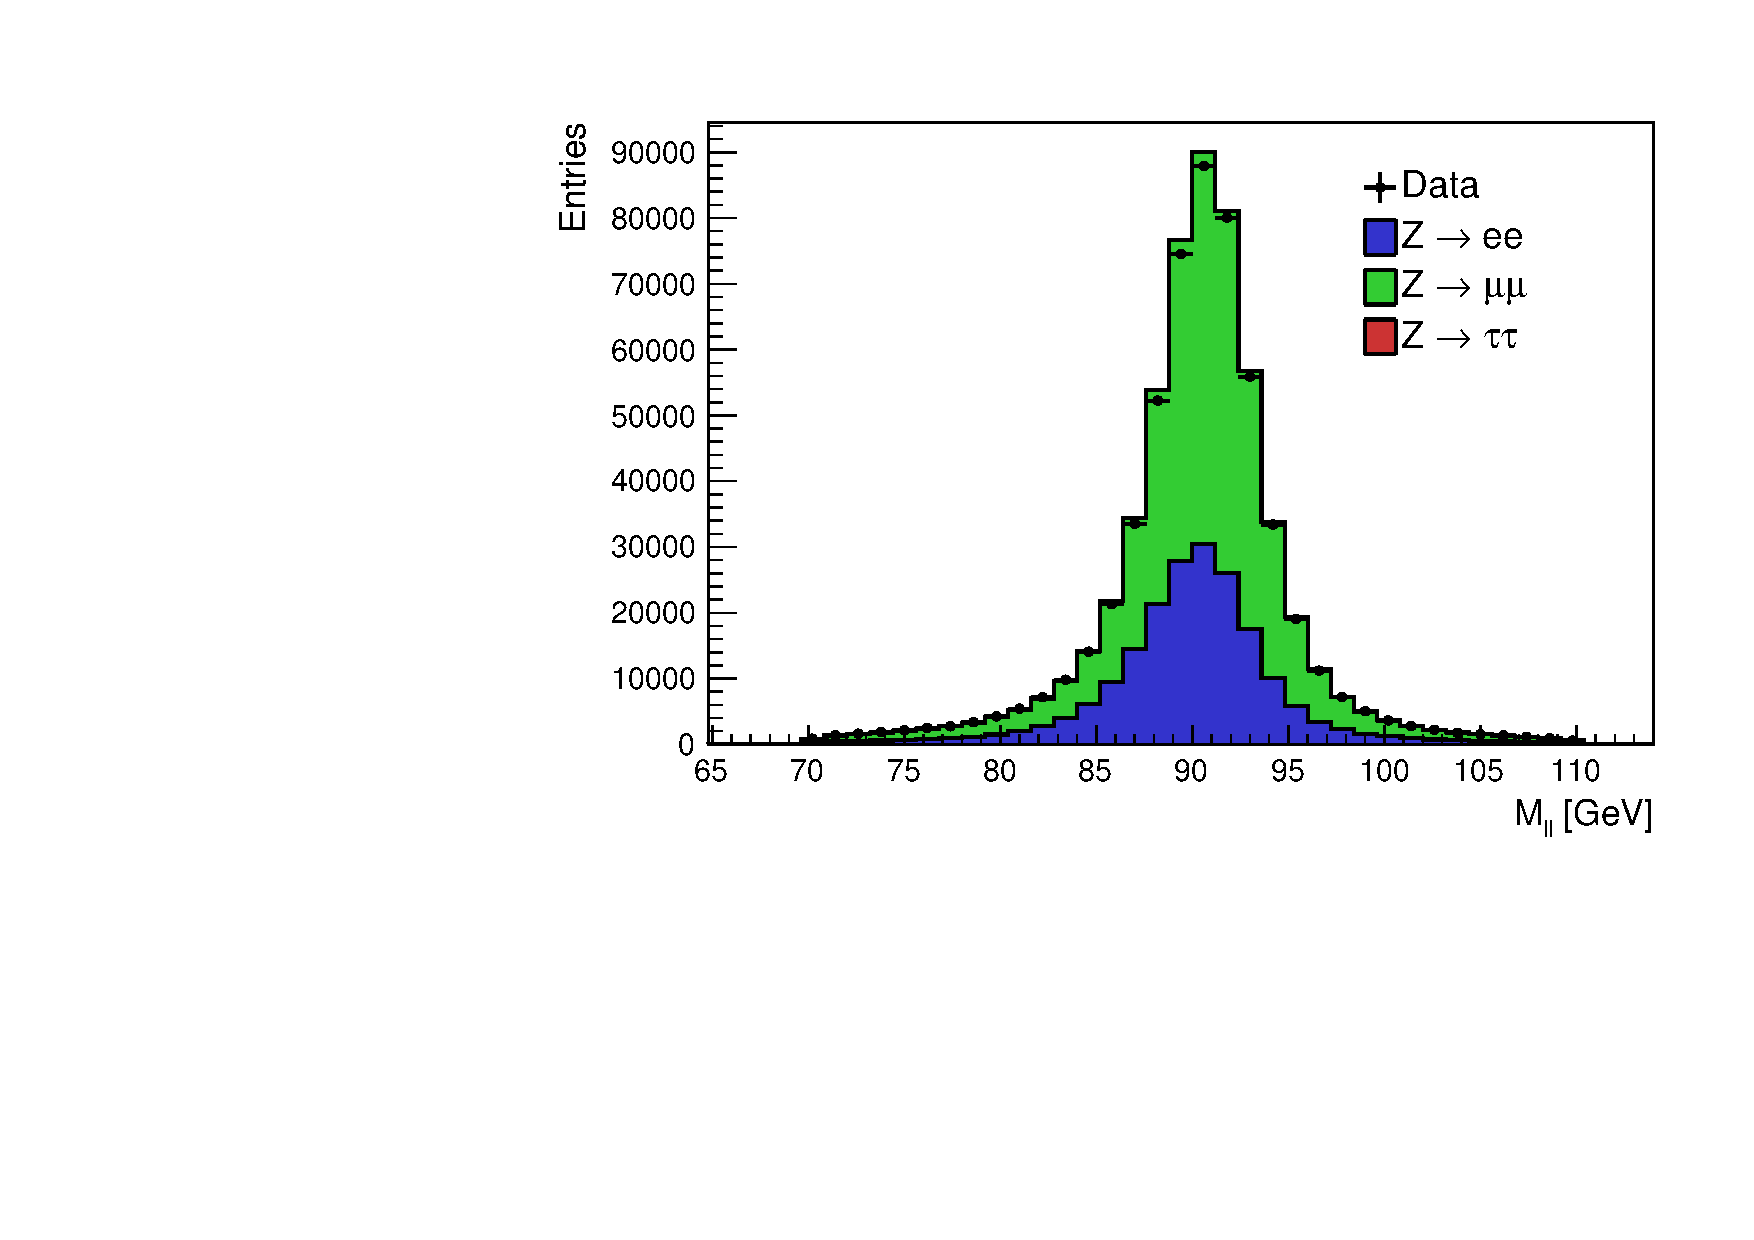
\includegraphics[width=\linewidth]{fig/vergleich_data_mc_final.pdf}
    \captionof{figure}{Comparison of measured data and MC simulation.}
	\label{fig:data_mc}
\end{center}


\subsection{Fitting the $Z$ mass}
Figure \ref{fig:fit} underlines the assumption from section 1.5, the best fit is provided by the convolution of a Gaussian and a Breit-Wigner distribution. 

One can determine the mass of the $Z$ boson and the decay width to: 

\begin{align}
M_Z &= (90.634 \pm 0.005) \ \text{GeV}\\
\Gamma &= (3.529 \pm 0.015) \ \text{GeV}
\end{align}

\begin{center}
	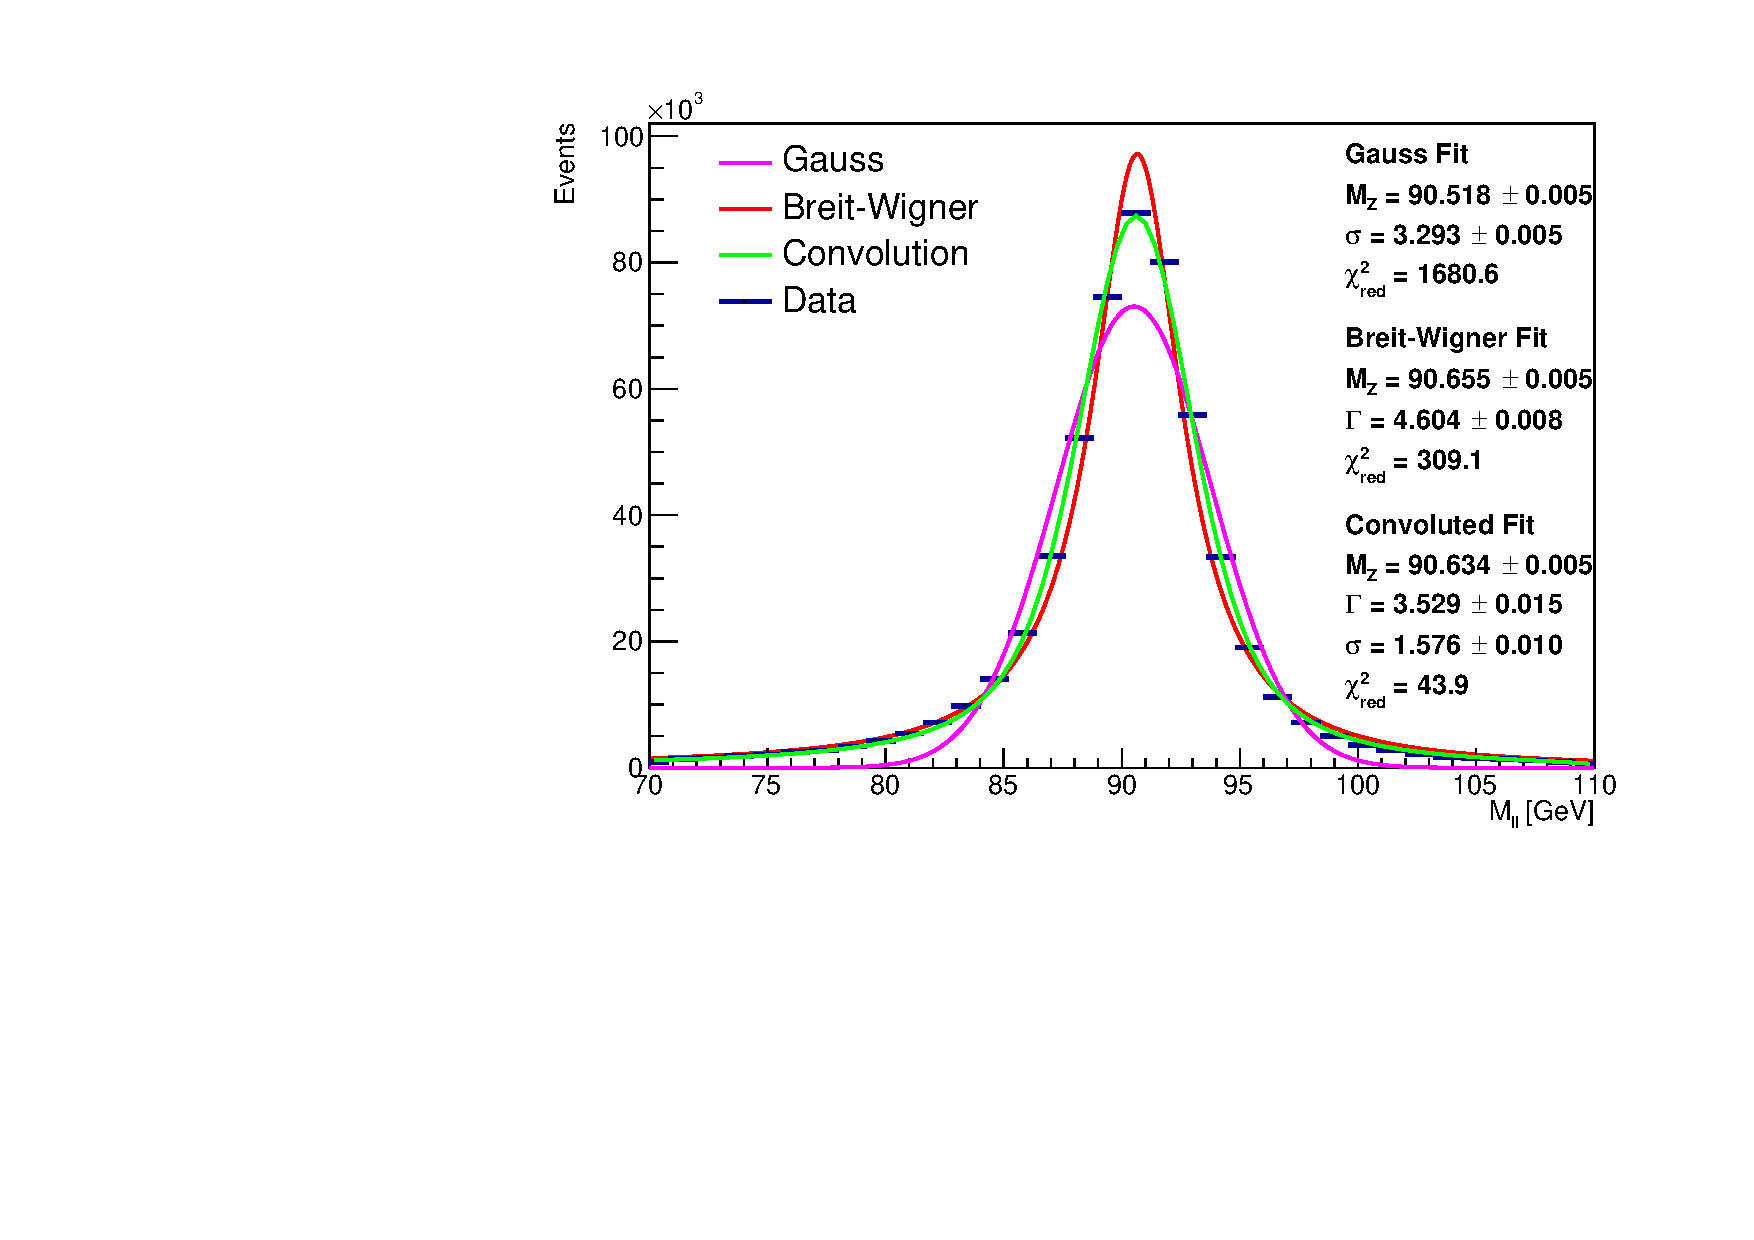
\includegraphics[width=\linewidth]{fig/invar_z_mass.pdf}
    \captionof{figure}{Different fits for $Z$ Boson mass.}
	\label{fig:fit}
\end{center}

A comparison of the results with the values (table \ref{table:zboson}) of the Particle Data Group yields differences of the order of $1$ GeV.
 
\begin{align}
\Delta M_Z &= (0.554 \pm 0.005) \ \text{GeV}\\
\Delta \Gamma &= (1.034 \pm 0.015) \ \text{GeV}
\end{align}
 
\subsection{Determining efficiencies}
For determining the efficiency of the identification, the tag and probe method (which was introduced earlier) is used.
The efficiency was computed for the MC simulation and for the real data and can be seen in figure \ref{fig:efficiency_comp}.

\begin{center}
    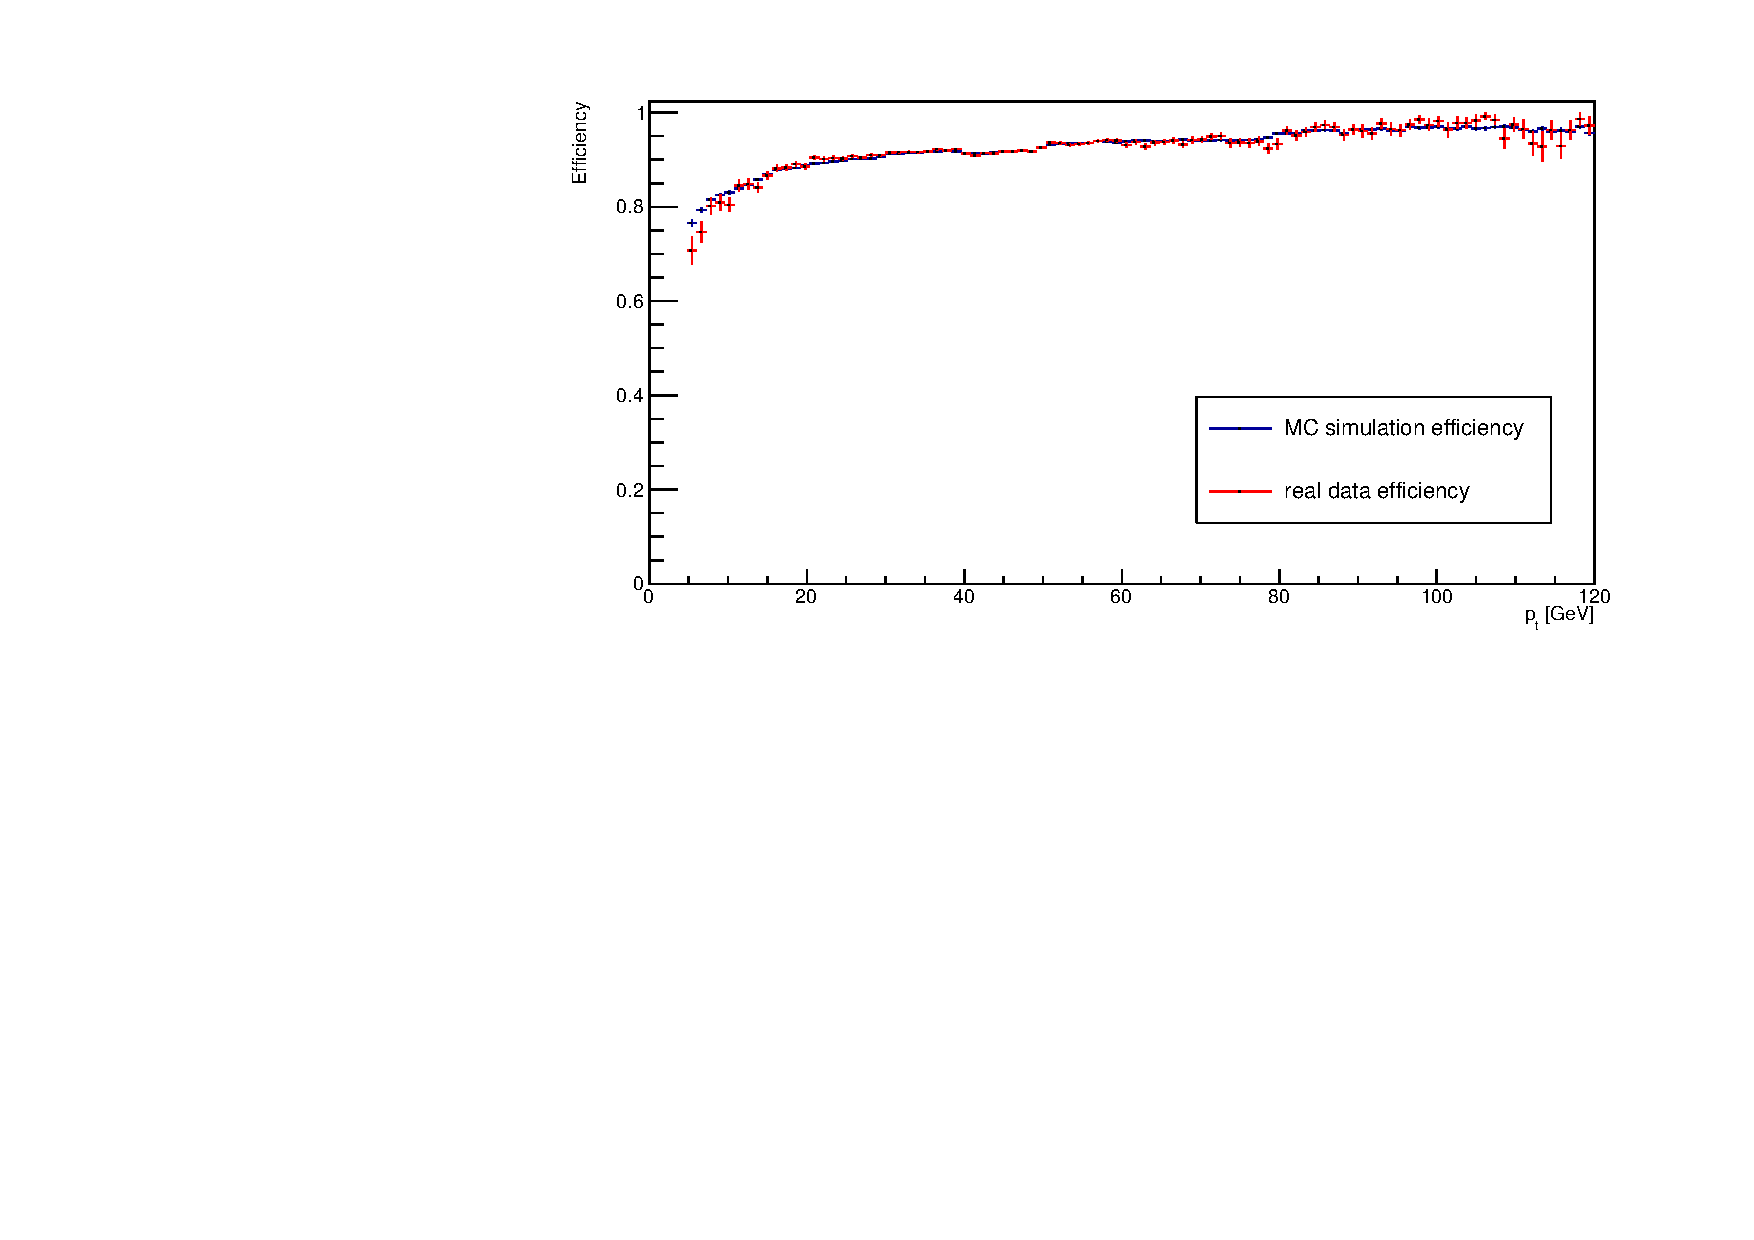
\includegraphics[width=1.1\linewidth]{fig/efficency_comparison_v2.pdf}
    \captionof{figure}{Comparison of the efficiencies of the MC simulation and the real data.}
    \label{fig:efficiency_comp}
\end{center}

With this method, one achieves an efficiency of approximately $90-95\%$ over the whole momentum range.

\section{Discussion}
The difference between the calculated result and the literature value of the $Z$ mass suggests that the errors were underestimated.
This is true in the lab course, because one neglects all sorts of error, only the error according to the fit is recognized.
Just from the size of the dataset, one assumes that the statistical error is reduced to a minimum (uncertainty scales with $\frac{1}{\sqrt{N}}$).
For the provided data one concludes that $\Delta_{stat.} \ll \Delta_{syst.}$.
Various factors contribute to systematic errors. 
The variance of the convoluted fit ($\sigma = (1.576 \pm 0.010)$ \si{GeV}) provides a first estimate of the energy resolution.
One of the prominent errors is the energy resolution in the calorimeter, which gets improved since the start of the ATLAS experiment. 
Another major part, which influences the uncertainty, comes from the usage of different triggers.
Firstly, to record an event, triggers have to be passed which work with an efficiency which could have been simulated. 
Later on, at the analysis of the data, one implements various filters (explained above).
With more time the used thresholds could be optimized.
As the difference of the values implies, a good understanding and recognition of the systematic uncertainties is necessary to improve the results.\\

Nevertheless, after making oneself familiar with \verb*+ROOT+ and the data, as well as with the Monte Carlo files, one was able to get insight into modern analysis in particle physics. 
The results, even without extensive error acknowledgment, verifies the used approach to identify the $Z$ boson mass as a valid method.  

%\newpage
\nocite{*}
\appendix
\printbibliography
\end{multicols}
\end{document}

